\documentclass{article}

\usepackage{arxiv}

\usepackage[utf8]{inputenc} % allow utf-8 input
\usepackage[T1]{fontenc}    % use 8-bit T1 fonts
\usepackage{hyperref}       % hyperlinks
\usepackage{url}            % simple URL typesetting
\usepackage{booktabs}       % professional-quality tables
\usepackage{amsfonts}       % blackboard math symbols
\usepackage{amsmath}
\usepackage{nicefrac}       % compact symbols for 1/2, etc.
\usepackage{microtype}      % microtypography
\usepackage{cleveref}       % smart cross-referencing
\usepackage{lipsum}         % Can be removed after putting your text content
\usepackage{graphicx}
\usepackage{natbib}
\usepackage{doi}
\usepackage{pythonhighlight}
\usepackage{graphicx}
\usepackage{subcaption}

\usepackage{polyglossia}
\setmainlanguage{english}
\setotherlanguage{polish}

\title{Training 1.58bit LLMs via Distillation}

% Here you can change the date presented in the paper title
%\date{September 9, 1985}
% Or remove it
%\date{}

\author{Łukasz Leszko \\
	\texttt{ll438580@student.mimuw.edu.pl} \\
	%% examples of more authors
	\And
	Filip Mateńko \\
	\texttt{f.matenko@student.uw.edu.pl} \\
}

% Uncomment to override  the `A preprint' in the header
% \renewcommand{\headeright}{Technical Report}
\renewcommand{\undertitle}{report}
\renewcommand{\shorttitle}{Training 1.58bit LLMs via Distillation}

%%% Add PDF metadata to help others organize their library
%%% Once the PDF is generated, you can check the metadata with
%%% $ pdfinfo template.pdf
\hypersetup{
pdftitle={A template for the arxiv style},
pdfsubject={q-bio.NC, q-bio.QM},
pdfauthor={Łukasz Leszko},
pdfkeywords={LLM, Distillatio, Quantization},
}

\begin{document}
\maketitle

\begin{abstract}
In this work, we propose an evaluation of LLMs distilled from a full-precision model down to 1.58-bit precision. Our evaluation will focus on the impact of different loss functions and quantization methods on the performance of the distilled model. We will try to validate claims that 1.58-bit quantization can achieve performance close to that of the full-precision models. The code is available at our GitHub repository\footnote{https://github.com/leszkolukasz/training-1.58bit-llms-via-distillation}. 
\end{abstract}


% keywords can be removed
% \keywords{First keyword \and Second keyword \and More}


\section{Introduction}
In recent years, we have observed rapid growth in Large Language Models (LLMs). They have expanded both in their capabilities and in size. 
Unlike other fields of machine learning, LLMs do not seem to follow the usual rules of overfitting when increasing the number of 
parameters. When properly trained, more parameters generally lead to better performance in this field. 

Unfortunately, as these models become larger, they require increasingly sophisticated hardware and computing power. Modern LLMs such as 
ChatGPT or DeepSeek-R1 demand multiple industrial-grade GPU accelerators to run efficiently. This requirement excludes individuals and 
organizations without access to such infrastructure from running these models locally, limiting full customization and integration.

Moreover, the energy consumption of human technology is considered one of the major issues of the 21st century. Data centers running LLMs 
consume enormous amounts of energy for both training and inference. One way to address this issue is through quantization - the process of 
reducing the precision of a model's parameters \cite{quantizationtechniques}.

Typically, parameters in LLMs are represented in 32-bit precision. The idea is to use lower precisions, such as 16-bit, 4-bit, 
or even 1-bit, to reduce the memory required to host and run the model. Many researchers around the world are approaching this task from 
different angles. Some claim to achieve performance close to that of unquantized LLMs \cite{wang2023bitnetscaling1bittransformers}. We 
decided to focus on the most extreme forms of quantization - reducing the representation to 1 bit (weights from set \(\{-1,1\}\)) - and compare it
with a 1.58-bit representation (weights from set \(\{-1,0,1\}\)). The second approach is less common but has already been introduced in BitNet 
b1.58 \cite{ma2024era1bitllmslarge}.

One possible method is to train the LLM in low precision from scratch. However, this approach, like any full training process, is
computationally expensive. Additionally, it poses challenges when computing gradients with respect to discrete-valued parameters.
An alternative is to take an existing high-precision model and distill it into a quantized model
\cite{du2024bitdistillerunleashingpotentialsub4bit}. The full-precision model serves as a teacher to a smaller, quantized student model. 
In our work, we aim to explore an approach similar to that used in FBI-LLM \cite{fbillm}, namely, knowledge distillation with Quantization Aware Training (QAT). In this work, the authors first binarize all 
linear transformer weights to 1-bit precision using a signum function - excluding embeddings, layer norms, and the head. They then introduce additional 
full-precision weights and biases for each binarized linear layer. These parameters, along with the head, become the only learnable 
components after bit quantization. The model is then distilled using a simple cross-entropy loss to align the responses of the student 
model with those of the teacher.

In our approach, we will explore both 1-bit and 1.58-bit quantizations. Additionally, we aim to experiment with different loss 
functions, such as Cross-entropy, KL divergence, Confidence-Aware KL divergence, and Wasserstein distance. These approaches have been investigated in various
prior works \cite{du2024bitdistillerunleashingpotentialsub4bit, boizard2025crosstokenizerdistillationuniversallogit}. Using KL divergence 
could better align the output distributions of the student and teacher models, as opposed to simply learning correct answers, which is 
the focus of cross-entropy loss. Moreover, Wasserstein distance may allow distillation even when the student and teacher use different tokenizers.

For future work, it would also be valuable to compare training from scratch with distillation-based approaches. Some researchers 
have also explored white-box distillation, which aims to mimic not only the final outputs but also the hidden states of the teacher 
model \cite{gu2024minillmknowledgedistillationlarge}.

\section{Experimental setup}

\subsection{Model}

Choosing model size is crucial for our experiments. Results from \cite{ma2024era1bitllmslarge} show that starting from 3B parameters, a 1.58-bit distilled student is able to match its teacher model. While our initial plan was to use a model in a similar size range (2-3B parameters), we quickly realized that the QAT process requires both student and teacher to be loaded into memory at the same time. This efficiently doubles the memory requirements and forces us to use a smaller model that can be run on our hardware. We decided to use SmolLM2 135M Instruct \cite{allal2025smollm2smolgoesbig}, which follows LLama2 architecture and whose 1.7B version outperforms many existing small LLMs, including Qwen2.5-1.5B and Llama3.2-1B. While we also tried other models like Qwen3 0.6B, we were not able to train them on our hardware due to memory constraints.

Both the student and the teacher will follow the SmolLM2 architecture. While it is possible to use different architectures for the student and the teacher (and when using Wasserstein loss, even architectures with different tokenizers), in our setup, the student will inherit the teacher's weights. Intuitively, this form of continued training from a pretrained LLM should allow the student to inherit the teacher's knowledge and speed up the training process. In \cite{fbillm}, the authors show that in the beginning of the training, continued training performs better than training from scratch, but it does not affect the performance of the distilled model in the long run. Our tests also suggest that continued training produces visible results more quickly than training from scratch.

\subsection{Quantization}

In our experiments, we consider both 1b and 1.58b quantization. As stated in \cite{du2024bitdistillerunleashingpotentialsub4bit}, sub-4-bit quantization cannot be done efficiently using Post-Training Quantization (PTQ), that is why we follow the QAT method, which is also what BitNet, OneBit \cite{onebit} and FBI does.

\subsubsection{1b quantization}

Given the weights \(W \in \mathcal{R}^{n \times m}\) the binarization can be formulated as:

\begin{gather*}
    Q_{1}(W) = \mathrm{Sign}(W - \alpha) \\
    \alpha = \frac{1}{nm}\sum_{ij}W_{ij} \\
    \mathrm{Sign}(W_{ij}) = \begin{cases}
        1& \text{if } W_{ij} > 0 \\
        -1  & \text{if } W_{ij} \le 0
    \end{cases}
\end{gather*}

In their original papers, both BitNet and OneBit follow this definition. FBI uses a very similar formula but without the \(\alpha\) parameter. We empirically tested that the absence of this parameter does not have large influence on the performance of the distilled model.


\subsubsection{1.58b quantization}

BitNet b1.58 adopted an absmean quantization function. It first scales the weight matrix by its average absolute value, and then round each value to
the nearest integer among \{-1, 0, +1\}:

\begin{gather*}
    Q_{1.58}(W) = \mathrm{RoundClip}(\frac{W}{\gamma + \epsilon}, -1, 1) \\
    \gamma = \frac{1}{nm}\sum_{ij}\left| W_{ij} \right| \\
    \mathrm{RoundClip}(x, a, b) = \mathrm{max}(a, \mathrm{min}(b, \mathrm{round}(x))),
\end{gather*}

where \(\epsilon\) makes sure to not divide by values close to \(0\).

\subsubsection{Implementation}

Because some operations used in quantization functions are non-differentiable, we use the Straight-Through Estimator (STE) method \cite{ste}, where the gradient of the output of the problematic function is used as an estimate for the gradient of the input.

As we use Pytorch for model development, using custom gradient propagation usually requires creating new \texttt{nn.Module}. However, we utilize a clever trick that does not require creation of new classes. Here is our implementation of 1.58b quantization:
\\
\begin{python}
def quantize_1_58b(
    w: torch.Tensor,
) -> torch.Tensor:
    scale = w.abs().mean() + EPSILON
    pre_round = w / scale
    return pre_round + (pre_round.round().clamp(-1, 1) - pre_round).detach()
\end{python}



One thing to note is that while the quantized weights, on disk, can be stored in a packed format, during training, we still need to store them in float16 format to compute gradients. Similarly, during inference, multiplying by a 1.58-bit quantized matrix does not require the \verb|MUL| operator; however, to benefit from that, we need to utilize custom hardware and kernels, which is outside of our expertise.

\subsection{BitLinear}

We follow the quantization process proposed in FBI, which replaces linear layers with a custom linear layer (BitLinear) that performs 1-bit or 1.58-bit quantization on weights during training. This approach allows us to easily add 1-bit and 1.58-bit quantization capabilities to any model with linear layers (not just transformers). In our experiments we compare three different BitLinear architectures from BitNet, FBI, and OneBit. Each BitLinear inherits from standard Pytorch \texttt{nn.Linear} layer. Let \(W, B\) denote the weight and bias parameters of the Linear layer, respectively.

\subsubsection{BitNet}

In BitNet activations are first transformed using absmax quantization into range \([-R, R]\), (\(R = 2^7\) in our case). The quantization proceeds as follows:

\begin{gather*}
    \tilde{x} = \mathrm{Clip}(\mathrm{LayerNorm}(x_{in}) \frac{R}{\gamma}, -R + \epsilon, R - \epsilon) \\
    \gamma = \left\lVert x_{in} \right\rVert_{\infty} \\
    \widetilde{W} = Q_b(W) \\
    x_{out} = \mathrm{Linear}(\tilde{x}, \widetilde{W}, B) \frac{\beta\gamma}{R} \\
    \beta = \frac{1}{nm}\left\lVert W \right\rVert_{1} 
\end{gather*}

\subsubsection{FBI}

Given learnable parameters \(\alpha, \beta \in \mathcal{R}^m\) the FBI BitLinear is defined as follows:

\begin{gather*}
    \widetilde{W}^{(1)} = Q_b(W) \\
    \widetilde{W}^{(2)}_{\cdot, j} = \alpha_j\widetilde{W}^{(1)}_{\cdot, j} + \beta_j \\
    x_{out} = \mathrm{Linear}(x_{in}, \widetilde{W}^{(2)}, B)
\end{gather*}

where \(W_{\cdot, j}\) denotes the j-th column of matrix. Parameters \(\alpha, \beta\) are initialized using corresponding teacher's weights \(W^t\) as follows:

\begin{gather*}
    \alpha_j = a_j \\
    \beta_j = \frac{1}{n}\sum^{n}_i\left|W^t_{ij} - a_j\right| \\
    a_j = \frac{1}{n}\sum^n_i W^t_{ij}
\end{gather*}

\subsubsection{OneBit}

Given learnable parameters \(g \in \mathcal{R}^n\), \(h \in \mathcal{R}^m\) the OneBit BitLinear is defined as follows:

\begin{gather*}
    \widetilde{W} = Q_b(W) \\
    \widetilde{W}^{(1)}_{i, \cdot} = g_i\widetilde{W}_{i, \cdot} \\
    \widetilde{W}^{(2)}_{\cdot, j} = h_j\widetilde{W}^{(1)}_{\cdot, j} \\
    x_{out} = \mathrm{LayerNorm}(\mathrm{Linear}(x_{in}, \widetilde{W}^{(2)}, B))
\end{gather*}

Parameters \(g, h\) are initialized to rank-1 approximation of \(|W_t|\) using SVD.

\subsection{Loss}

Most common losses used in distillation are cross-entropy and Kullback–Leibler divergence. In our tests we will also utilize two other losses:  Confidence-Aware KL divergence and Wasserstein Distance.

\subsubsection{Confidence-Aware KL}

Let \(P_S, P_T, D_{KL}\) denote student output probabilities, teacher output probabilities and Kullback–Leibler divergence measure, respectively. When measuring distance between distributions, one can do this in two ways:

\begin{itemize}
    \item Forward KL -- \(D_{KL} (P_T \,||\, P_S)\)
    \item Reverse KL -- \(D_{KL} (P_S \,||\, P_T)\)
\end{itemize}

According to \cite{du2024bitdistillerunleashingpotentialsub4bit}, Forward KL loss is superior at guiding models in general text generation like summarization while Reverse KL is better for instruction tuning. With that in mind, authors of \cite{du2024bitdistillerunleashingpotentialsub4bit} propose a blend of those two losses, more specifically:

\begin{gather*}
    D_{CAKL} (P_T \,||\, P_S) = \gamma D_{KL} (P_S \,||\, P_T) + (1 - \gamma) D_{KL} (P_T \,||\, P_S) \\
    \gamma = \mathbb{E}_{(x, y) \sim D}\left[\frac{1}{|\{y\}|}\sum^{|\{y\}|}_i P_T(y_i | x, y_{<i}) \right]
\end{gather*}

Intuitively, when teacher is confident on training data, CAKL will prefer mode-seeking behaviour, but when teacher is not certain, then mode-covering behaviour.

\subsubsection{Wasserstein Distance}

Wasserstein distance stems from optimal transport theory. It minimizes transport costs between sampled points from
all possible couplings. With some assumptions \cite{boizard2025crosstokenizerdistillationuniversallogit}, it can be simplified to closed form:

\begin{gather*}
    \mathcal{W} = \sum^s_{t=1}\sum^d_{i=1}\left|P_S(x^S_{\sigma^S(i)} | x^S_{<t}) - P_T(x^T_{\sigma^T(i)} | x^T_{<t})\right|
\end{gather*}

where \(s\) is sequence length, \(d\) vocabulary size, \(\sigma\) permutation that sorts in decreasing order probabilities of student or teacher. This formulation allows for cross-tokenizer training.

\subsection{Training}

To train selected models we will utilize Pytorch Lightning framework. The training is performed on 4 GPUs. Two of them are L4 accessed via Google Cloud. We use the hyperparameter from table \ref{table:hypr}.

\begin{table}[ht]
  \centering
  \begin{tabular}{lc}
    \toprule
    Hyperparameter & Value \\
    \midrule
    Sequence Length        & 1024 \\
    GA frequency & 16 \\
    Learning Rate          & $10^{-3}$ \\
    Optimizer              & AdamW \\
    Scheduler              & CosineAnnealingLR \\
    Weight Decay           & 0.1 \\
    Total Training Steps   & 16,000 \\
    Gradient Clipping      & 1.0 \\
    Precision              & bfloat16 \\
    \bottomrule
  \end{tabular}
  \vspace{0.5em}
  \caption{Hyperparameters used for LLM training}
   \label{table:hypr}
\end{table}

These are the hyperparameters we found to work the best. In Figure \ref{fig:lr}, one can see how learning rate influences the loss. Since we were severely limited by the VRAM of the available devices, we have decided to use Gradient Accumulation (GA) technique. Batch sizes differed among different training sessions, since the presented techniques differ by memory requirements, and the used GPUs had different memory.

\begin{figure}[ht]
  \centering
  \begin{subfigure}[b]{0.3\textwidth}
    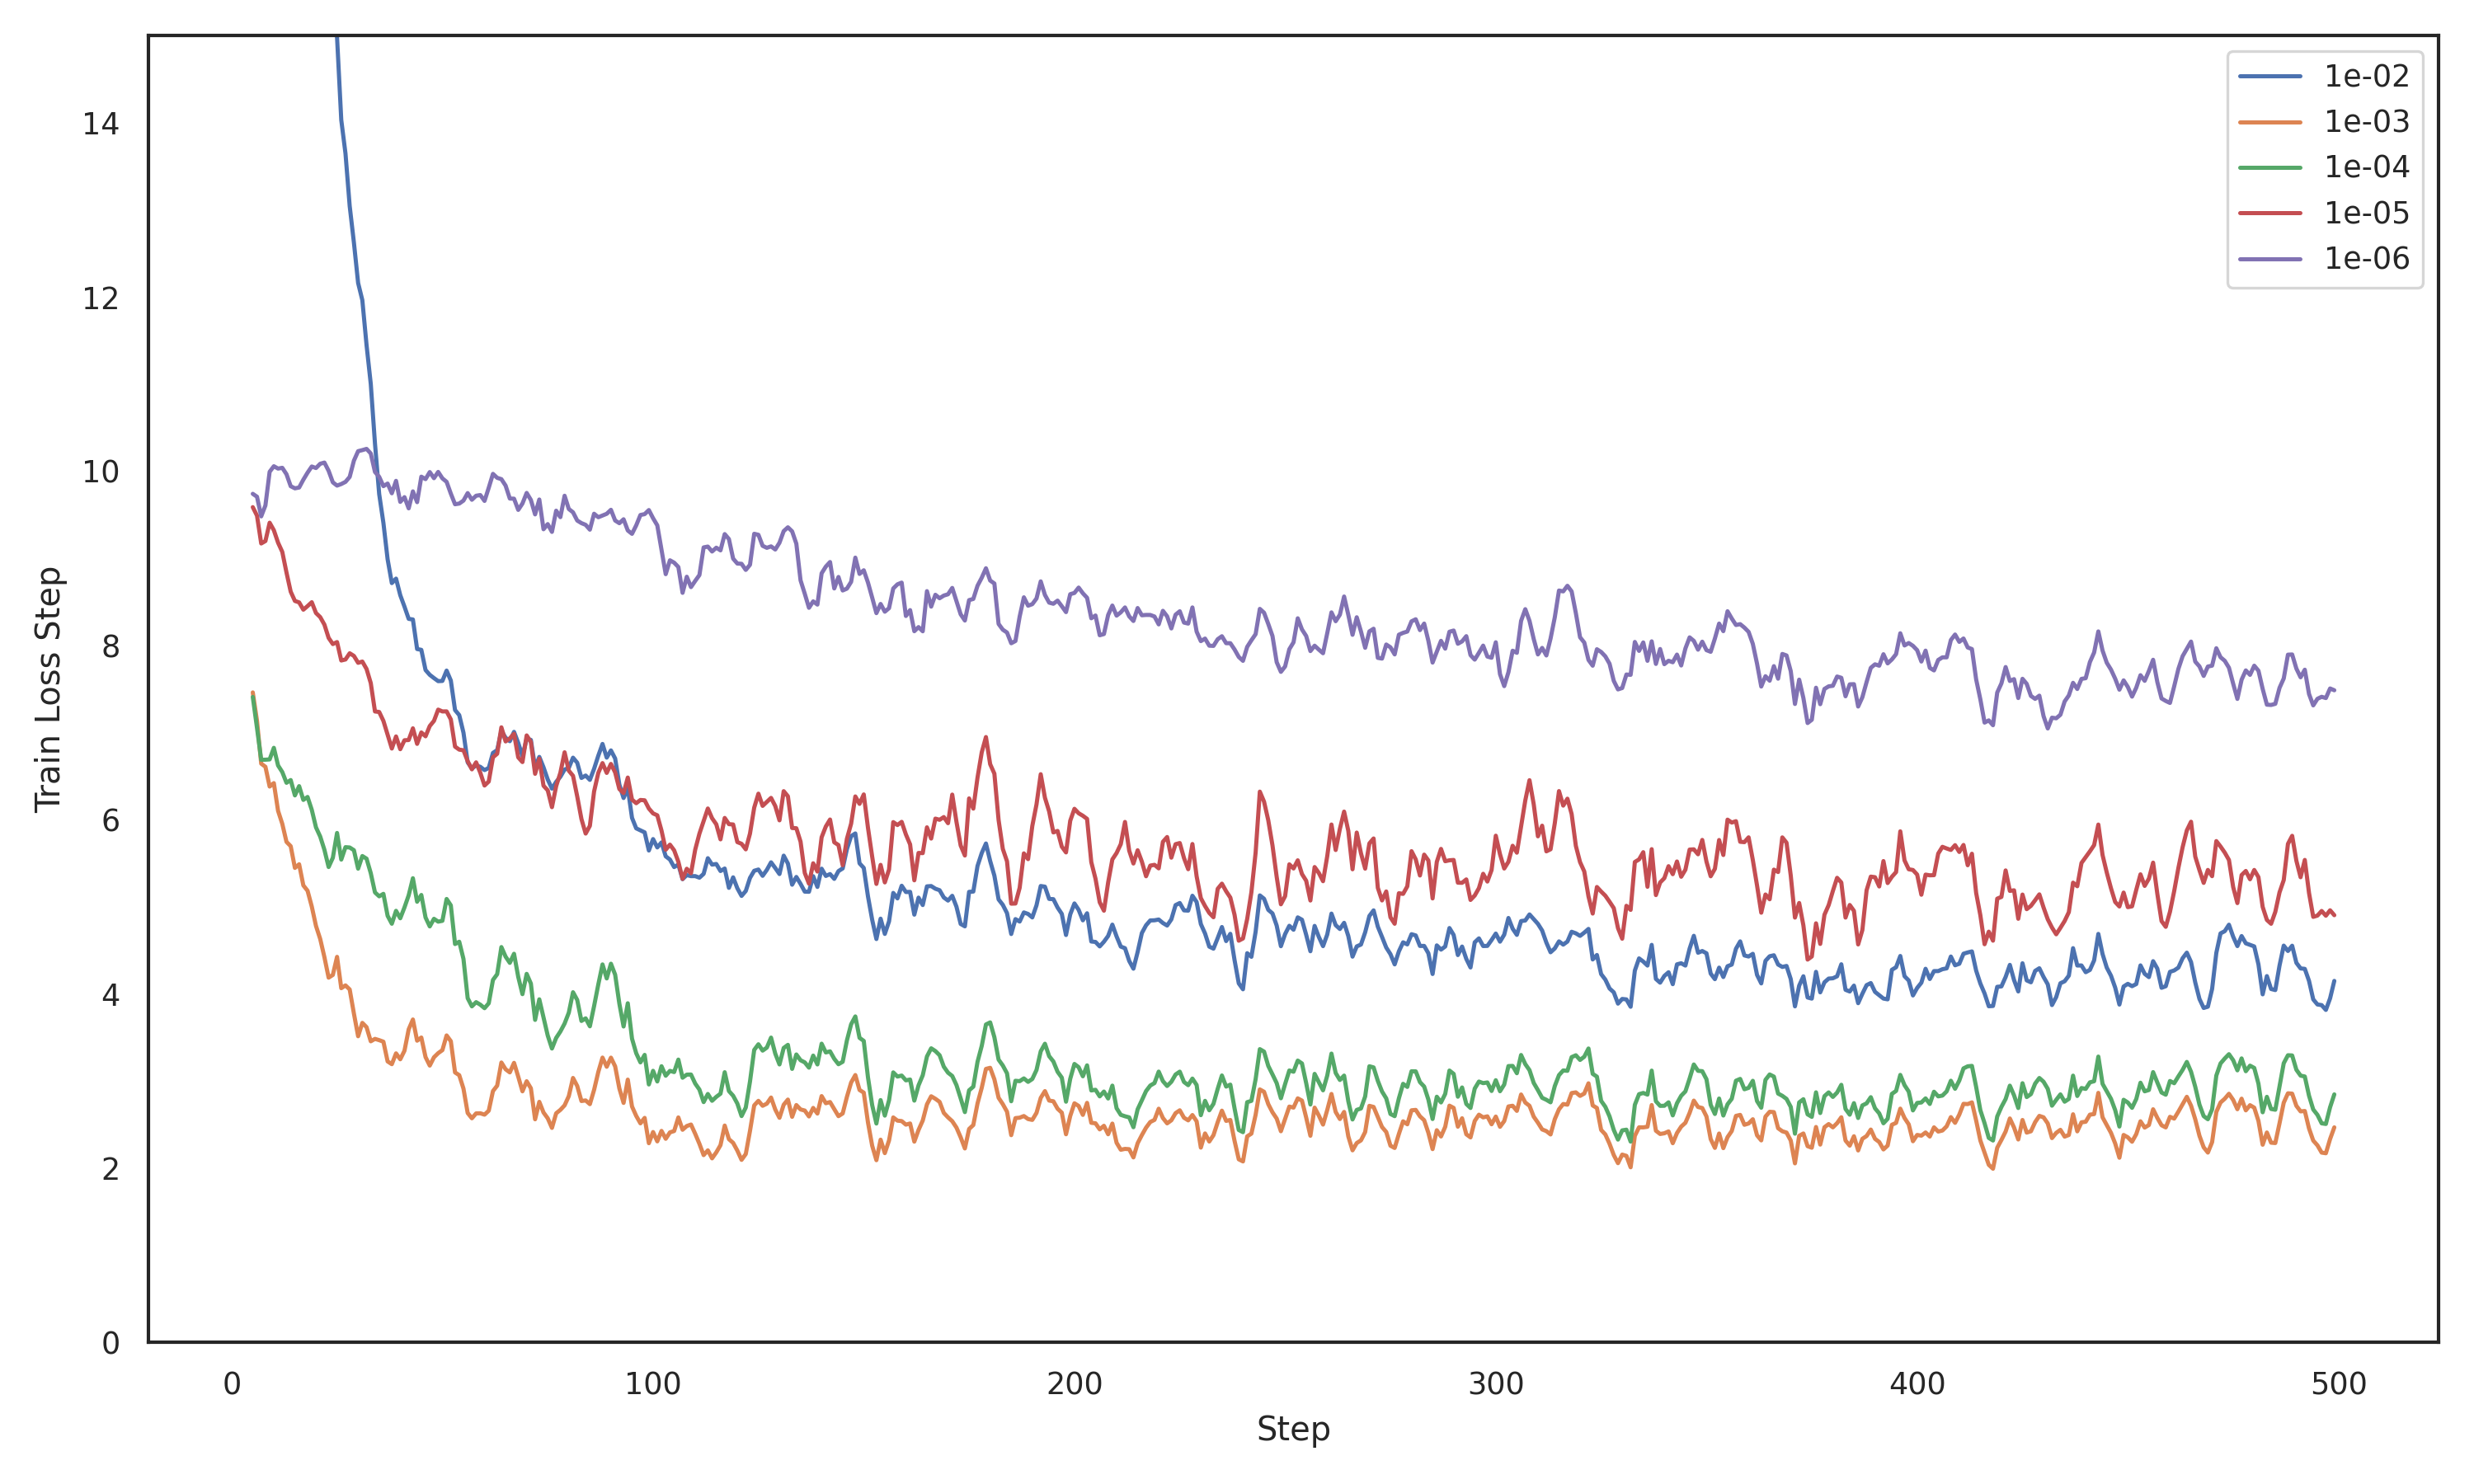
\includegraphics[width=\linewidth]{../data/plots/BitNet_lr.png}
    \caption{BitNet}
  \end{subfigure}
  \hfill
  \begin{subfigure}[b]{0.3\textwidth}
    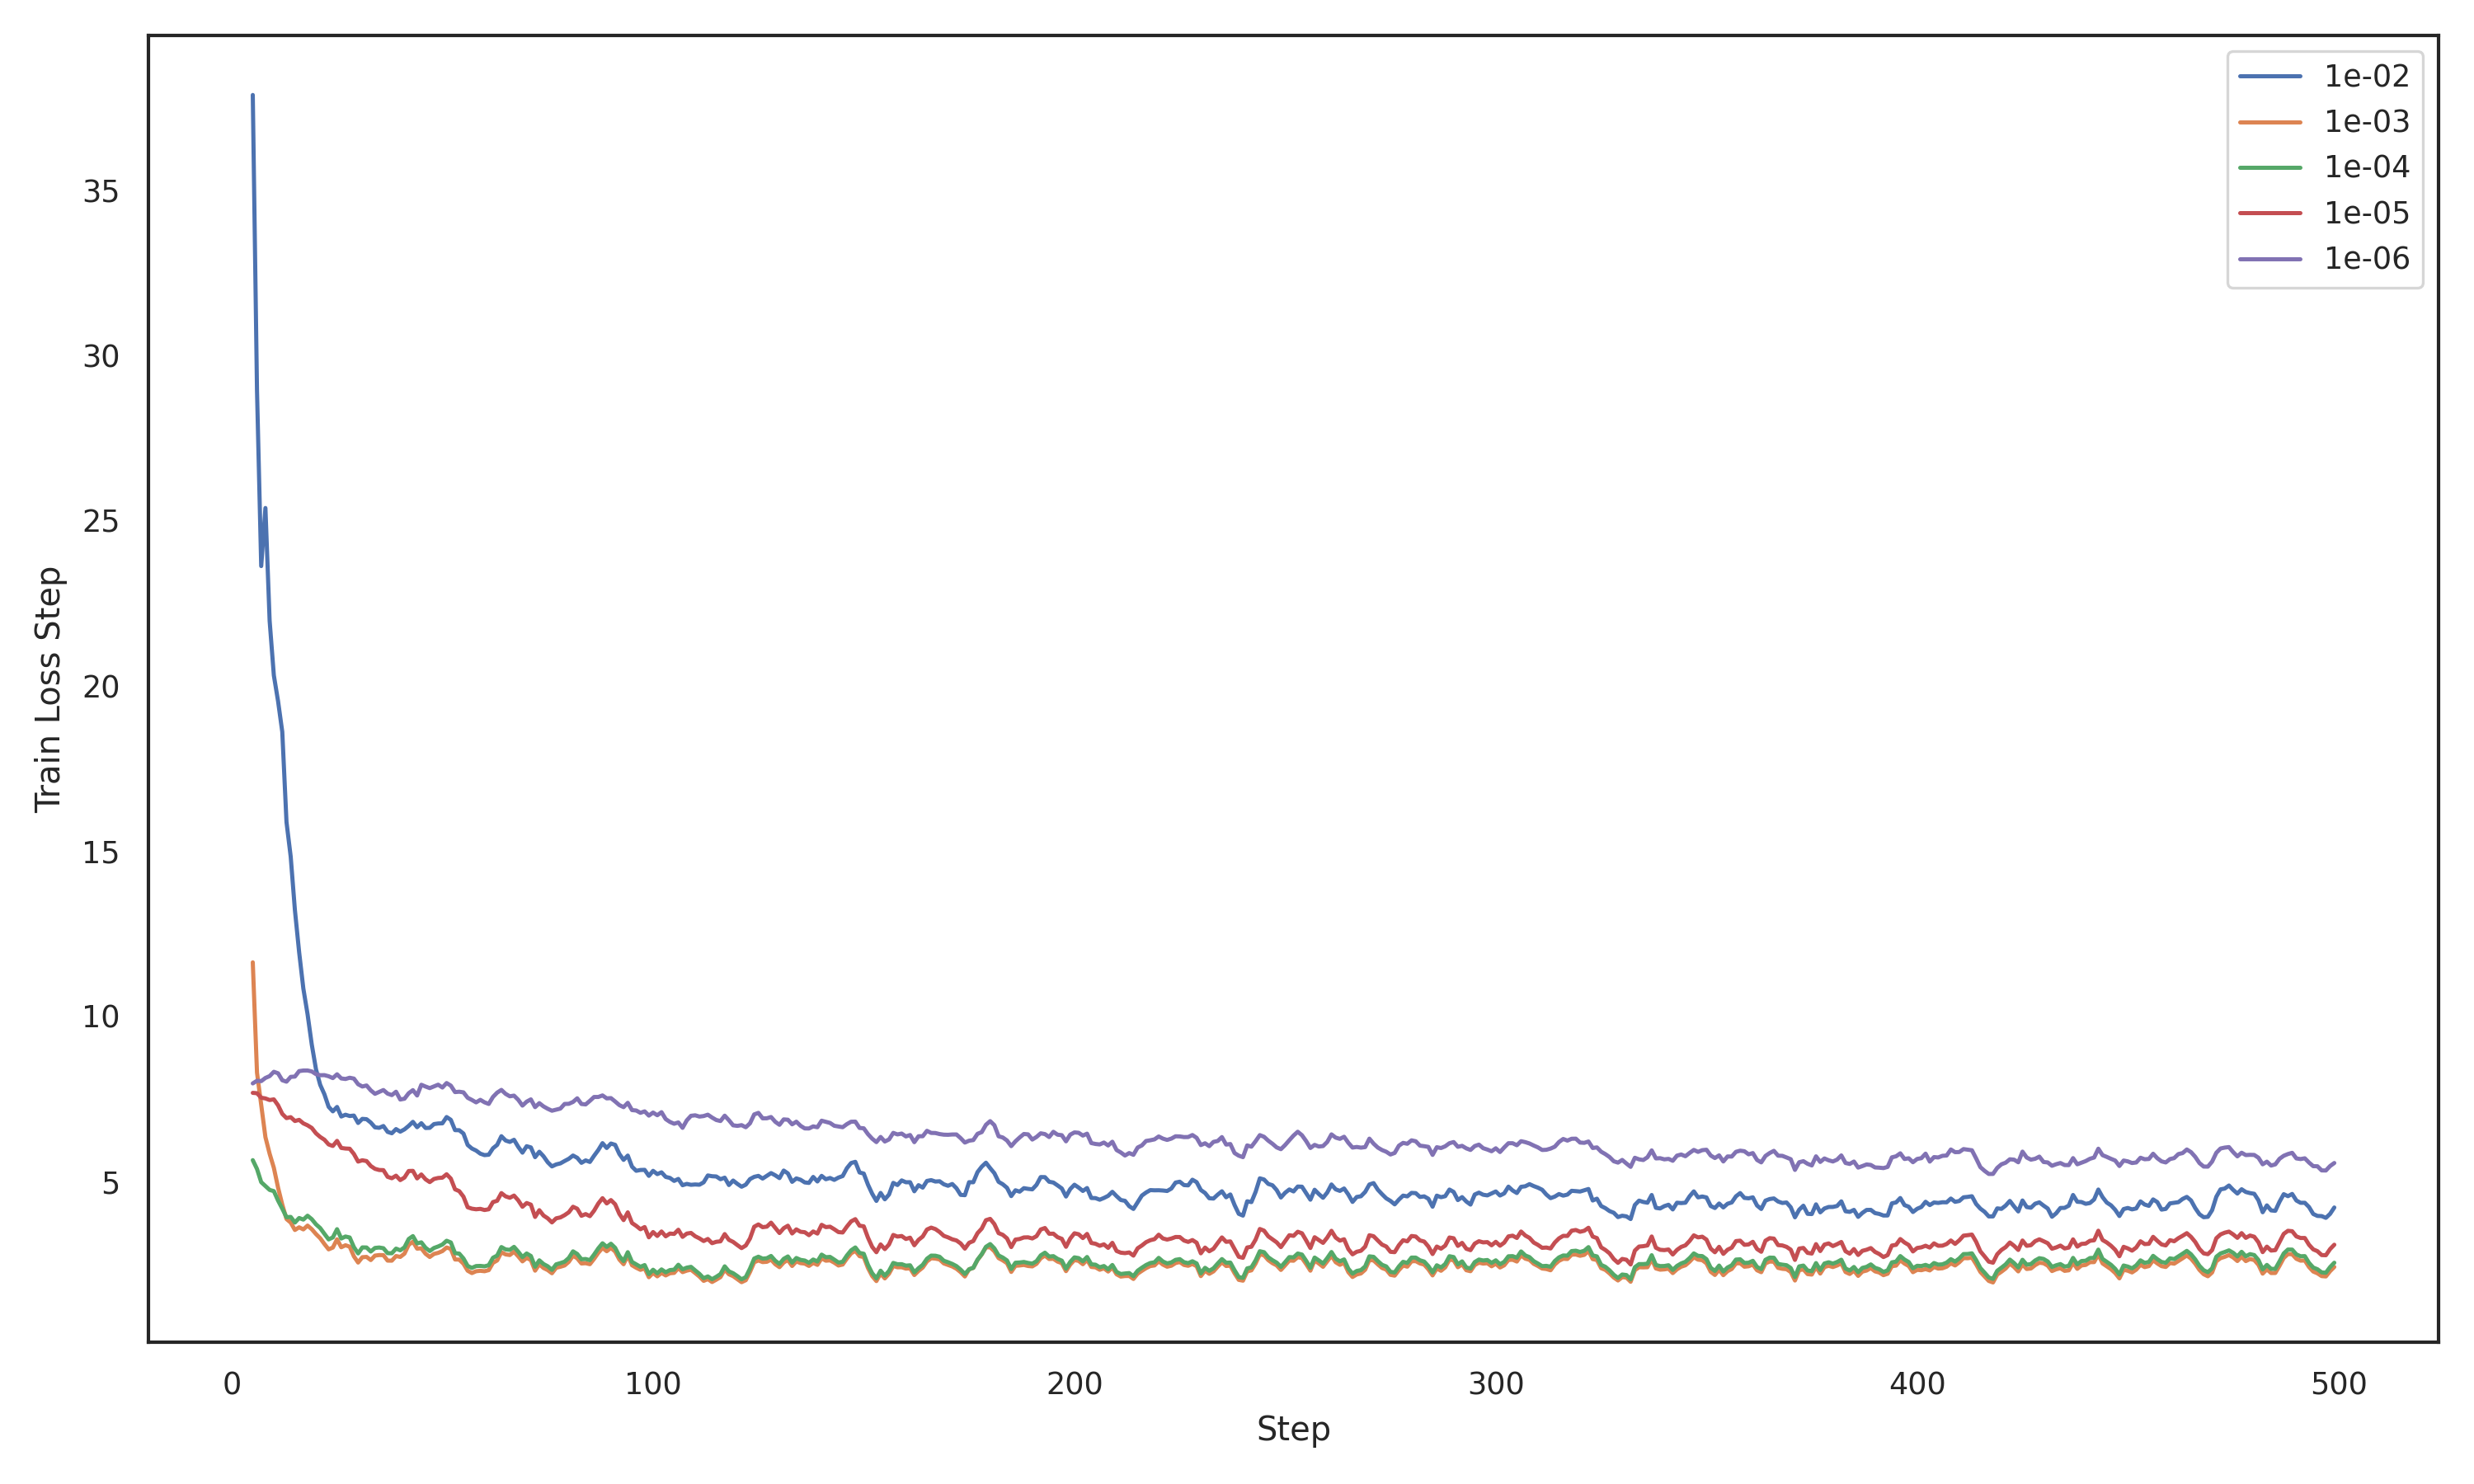
\includegraphics[width=\linewidth]{../data/plots/OneBit_lr.png}
    \caption{OneBit}
  \end{subfigure}
  \hfill
  \begin{subfigure}[b]{0.3\textwidth}
    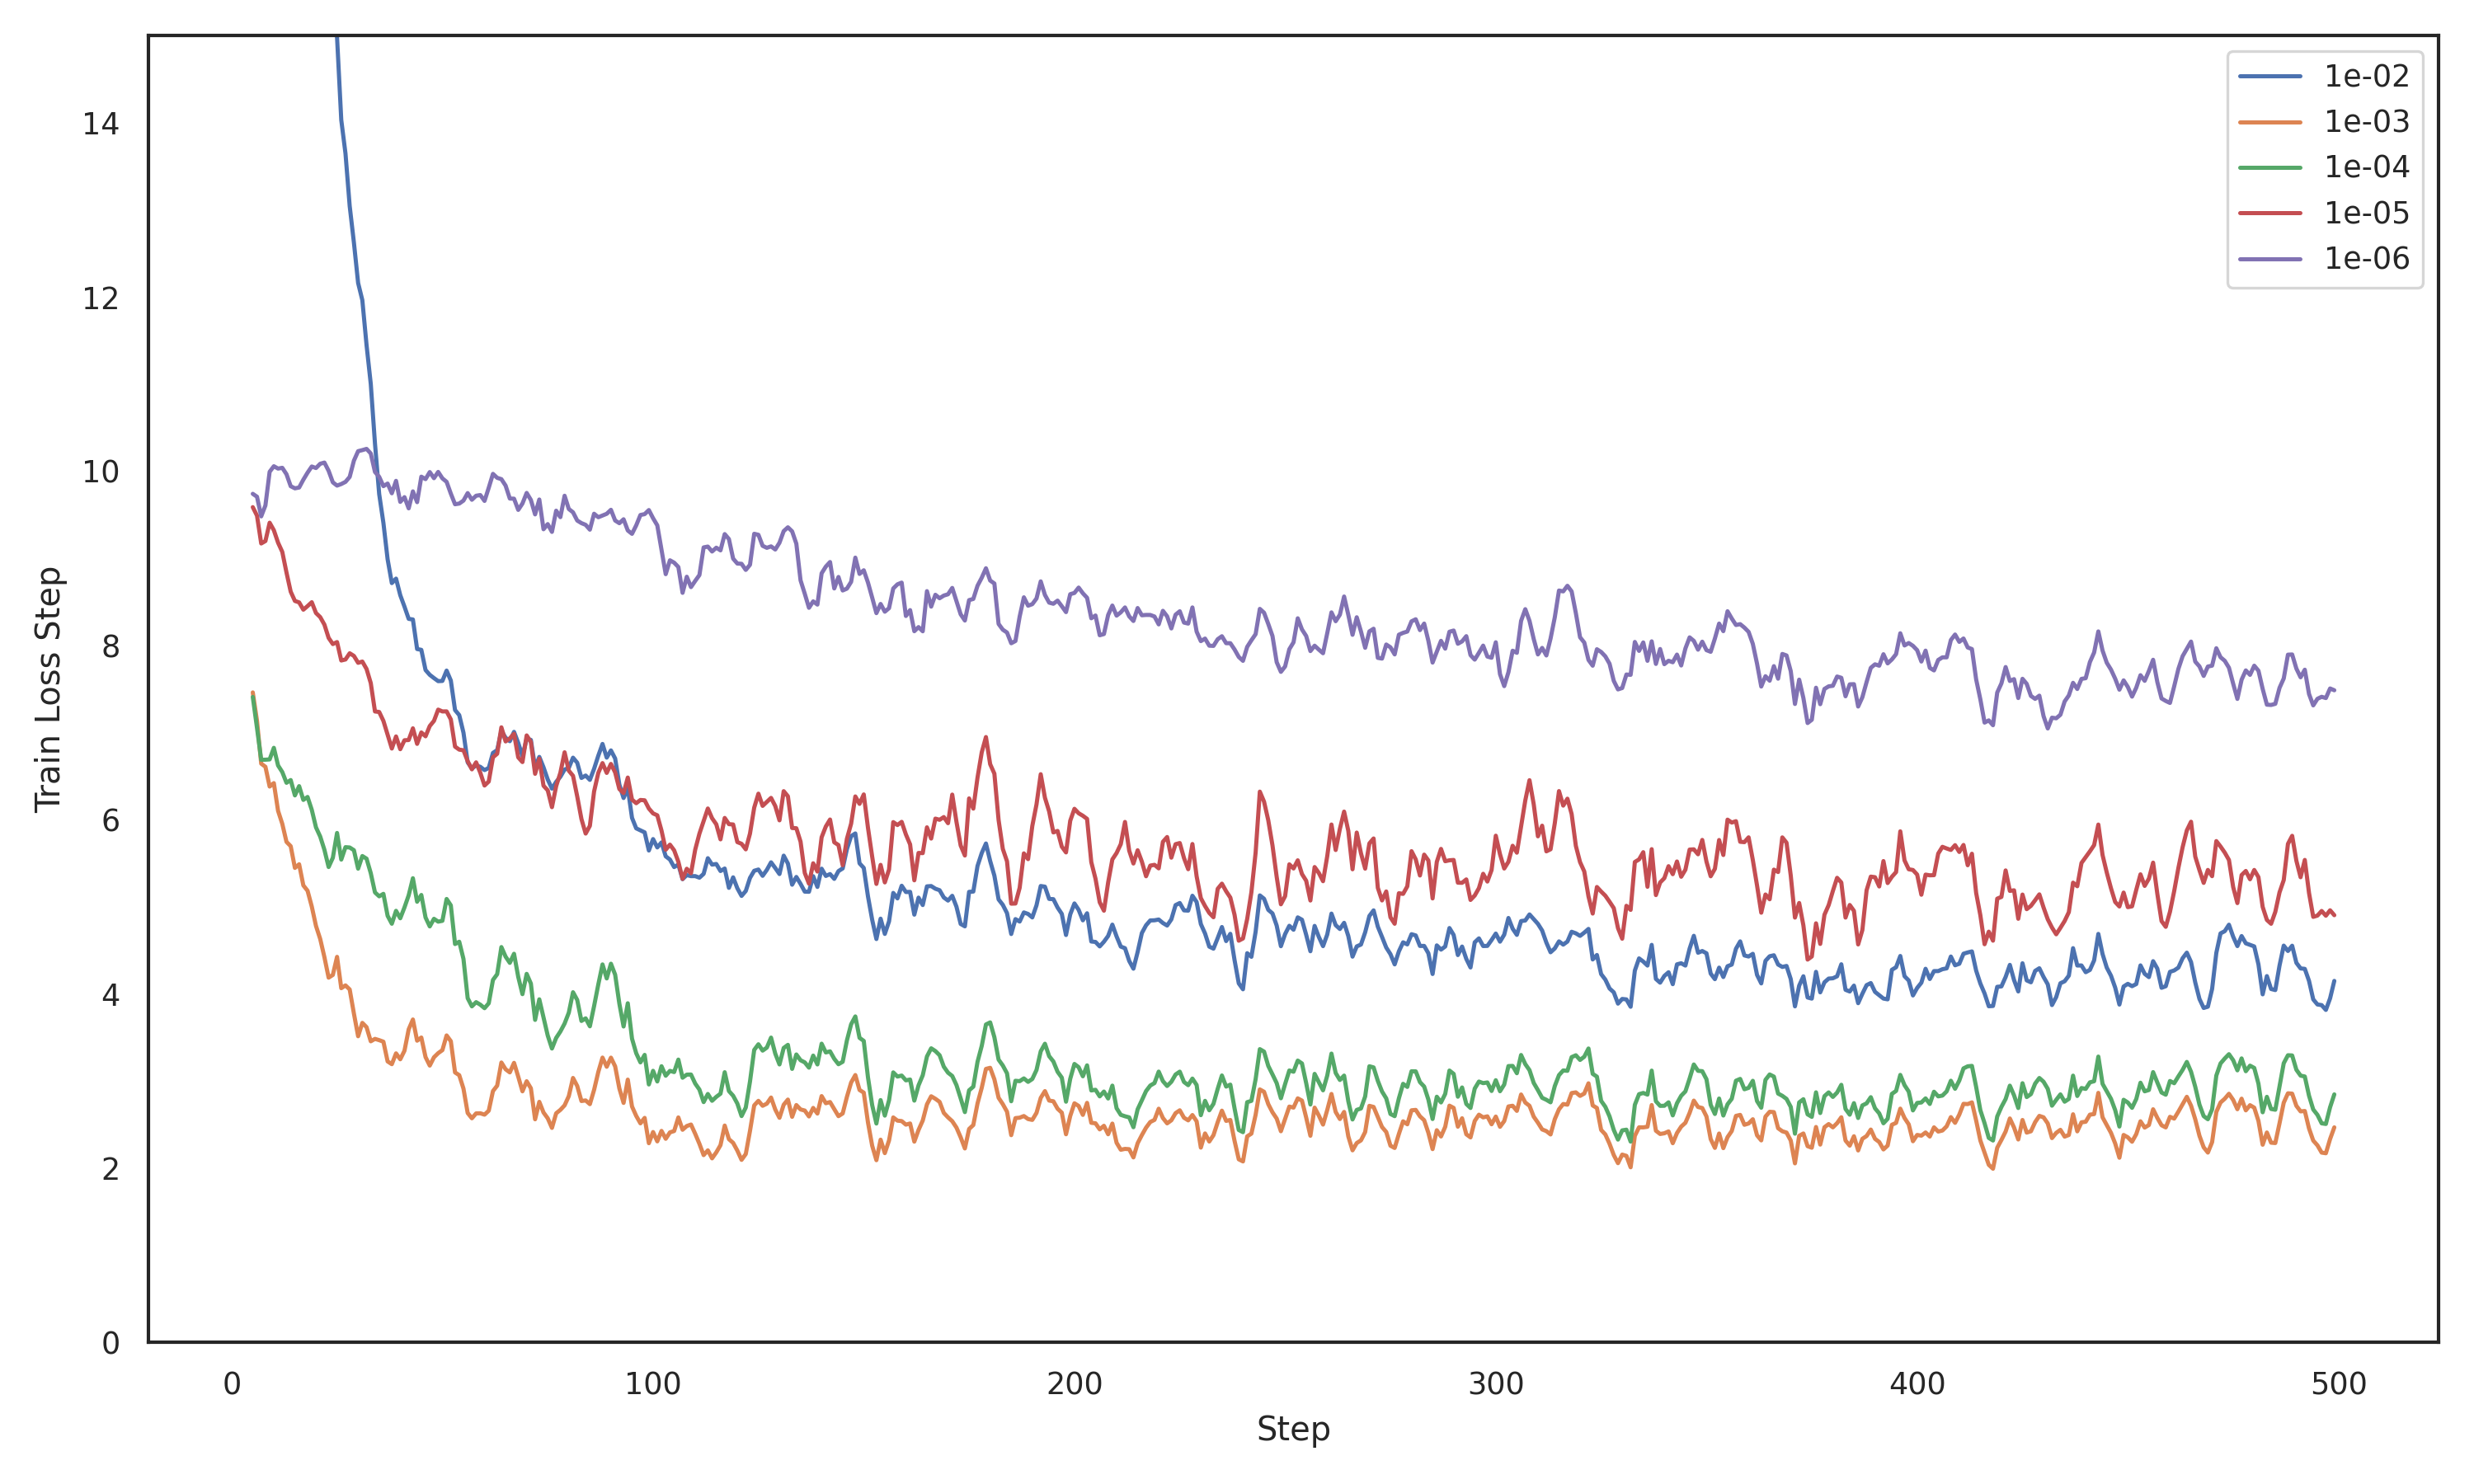
\includegraphics[width=\linewidth]{../data/plots/BitNet_lr.png}
    \caption{FBI}
  \end{subfigure}
  \vspace{0.5em}
  \caption{Influence of learning rate on loss}
  \label{fig:lr}
\end{figure}


We use Amber dataset \cite{llm360}. The Amber dataset is an agglomeration of RefinedWeb \cite{refinedweb}, StarCoder \cite{starcoder}, and RedPajama-v1 \cite{redpajama} and contains 1.26 trillion tokens. We only utilize a small 100k sample subset of this dataset.

In addition, as noted in the FBI-LLM paper, training extremely quantized models with distillation may be unstable and result in models that fail to converge. We will monitor this stability by tracking the gradient norm and the flip-flop rate \cite{flipflop}, which is the percentage of quantized weights that changed sign during a training step.

\section{Results}

Initially, we planned to quantize all linear layers except for embeddings and head as suggested by the authors of FBI. This led to slower model convergence and because of time and hardware constraints, we decided to quantize only some layers.

The question arises: which layers should be quantized? We hypothesized that it is best to quantize the least important layers in the model. To determine the importance of layer, we use the heuristics introduced in \cite{dumitru2024layerwisequantizationpragmaticeffective}, that is: Layer Input Modification (LIM) and z-score distribution (ZD).

\subsubsection{LIM}

Let \(L\) be a layer in model, \(L^I\) its input and \(L^O\) its output. Then LIM score is defined as:

\begin{equation*}
    \mathrm{LIM}(L) = -\frac{L^IL^O}{\left\lVert L^I \right\rVert\left\lVert L^O \right\rVert}
\end{equation*}

which is negative cosine similarity between the input and output of the given layer. This formula requires input and output to be of the same shape, which is why in the importance analysis, we treated FFN as a single layer. Similarly attention block was also treated as a single layer as SmolLM2 135M Instruct uses multi-query attention, and not all of its projection layers have the dimension of the embedding.

\subsubsection{ZD}

The z-score of a weight \(w_i\) in layer \(L\) is defined as:

\begin{equation*}
    z_i = \frac{w_i - \mu}{\sigma}
\end{equation*}

where \(\mu\) is mean of weights in layer, and \(\sigma\) their standard deviation. Then ZD is defined as:

\begin{equation*}
    ZD(L) = \frac{\sum_{w_i} [z_i > 1]}{N}
\end{equation*}

where N is the number of weights in the layer. The formula describes the ratio of weights with z-score greater than 1 to the total number of weights.

Both LIM and ZD score showed that the most important are the FFN layers and the least important are the attention layers. That is why we first quantized the attention layers, thinking that they would result in the smallest model degradation. Surprisingly, tests show that it is better to quantize the most important layers in the model as shown on \ref{fig:layers}. We speculate that the attention layers contain information that is harder to quantize.

\begin{figure}[ht]
  \centering
  \begin{subfigure}[b]{0.45\textwidth}
    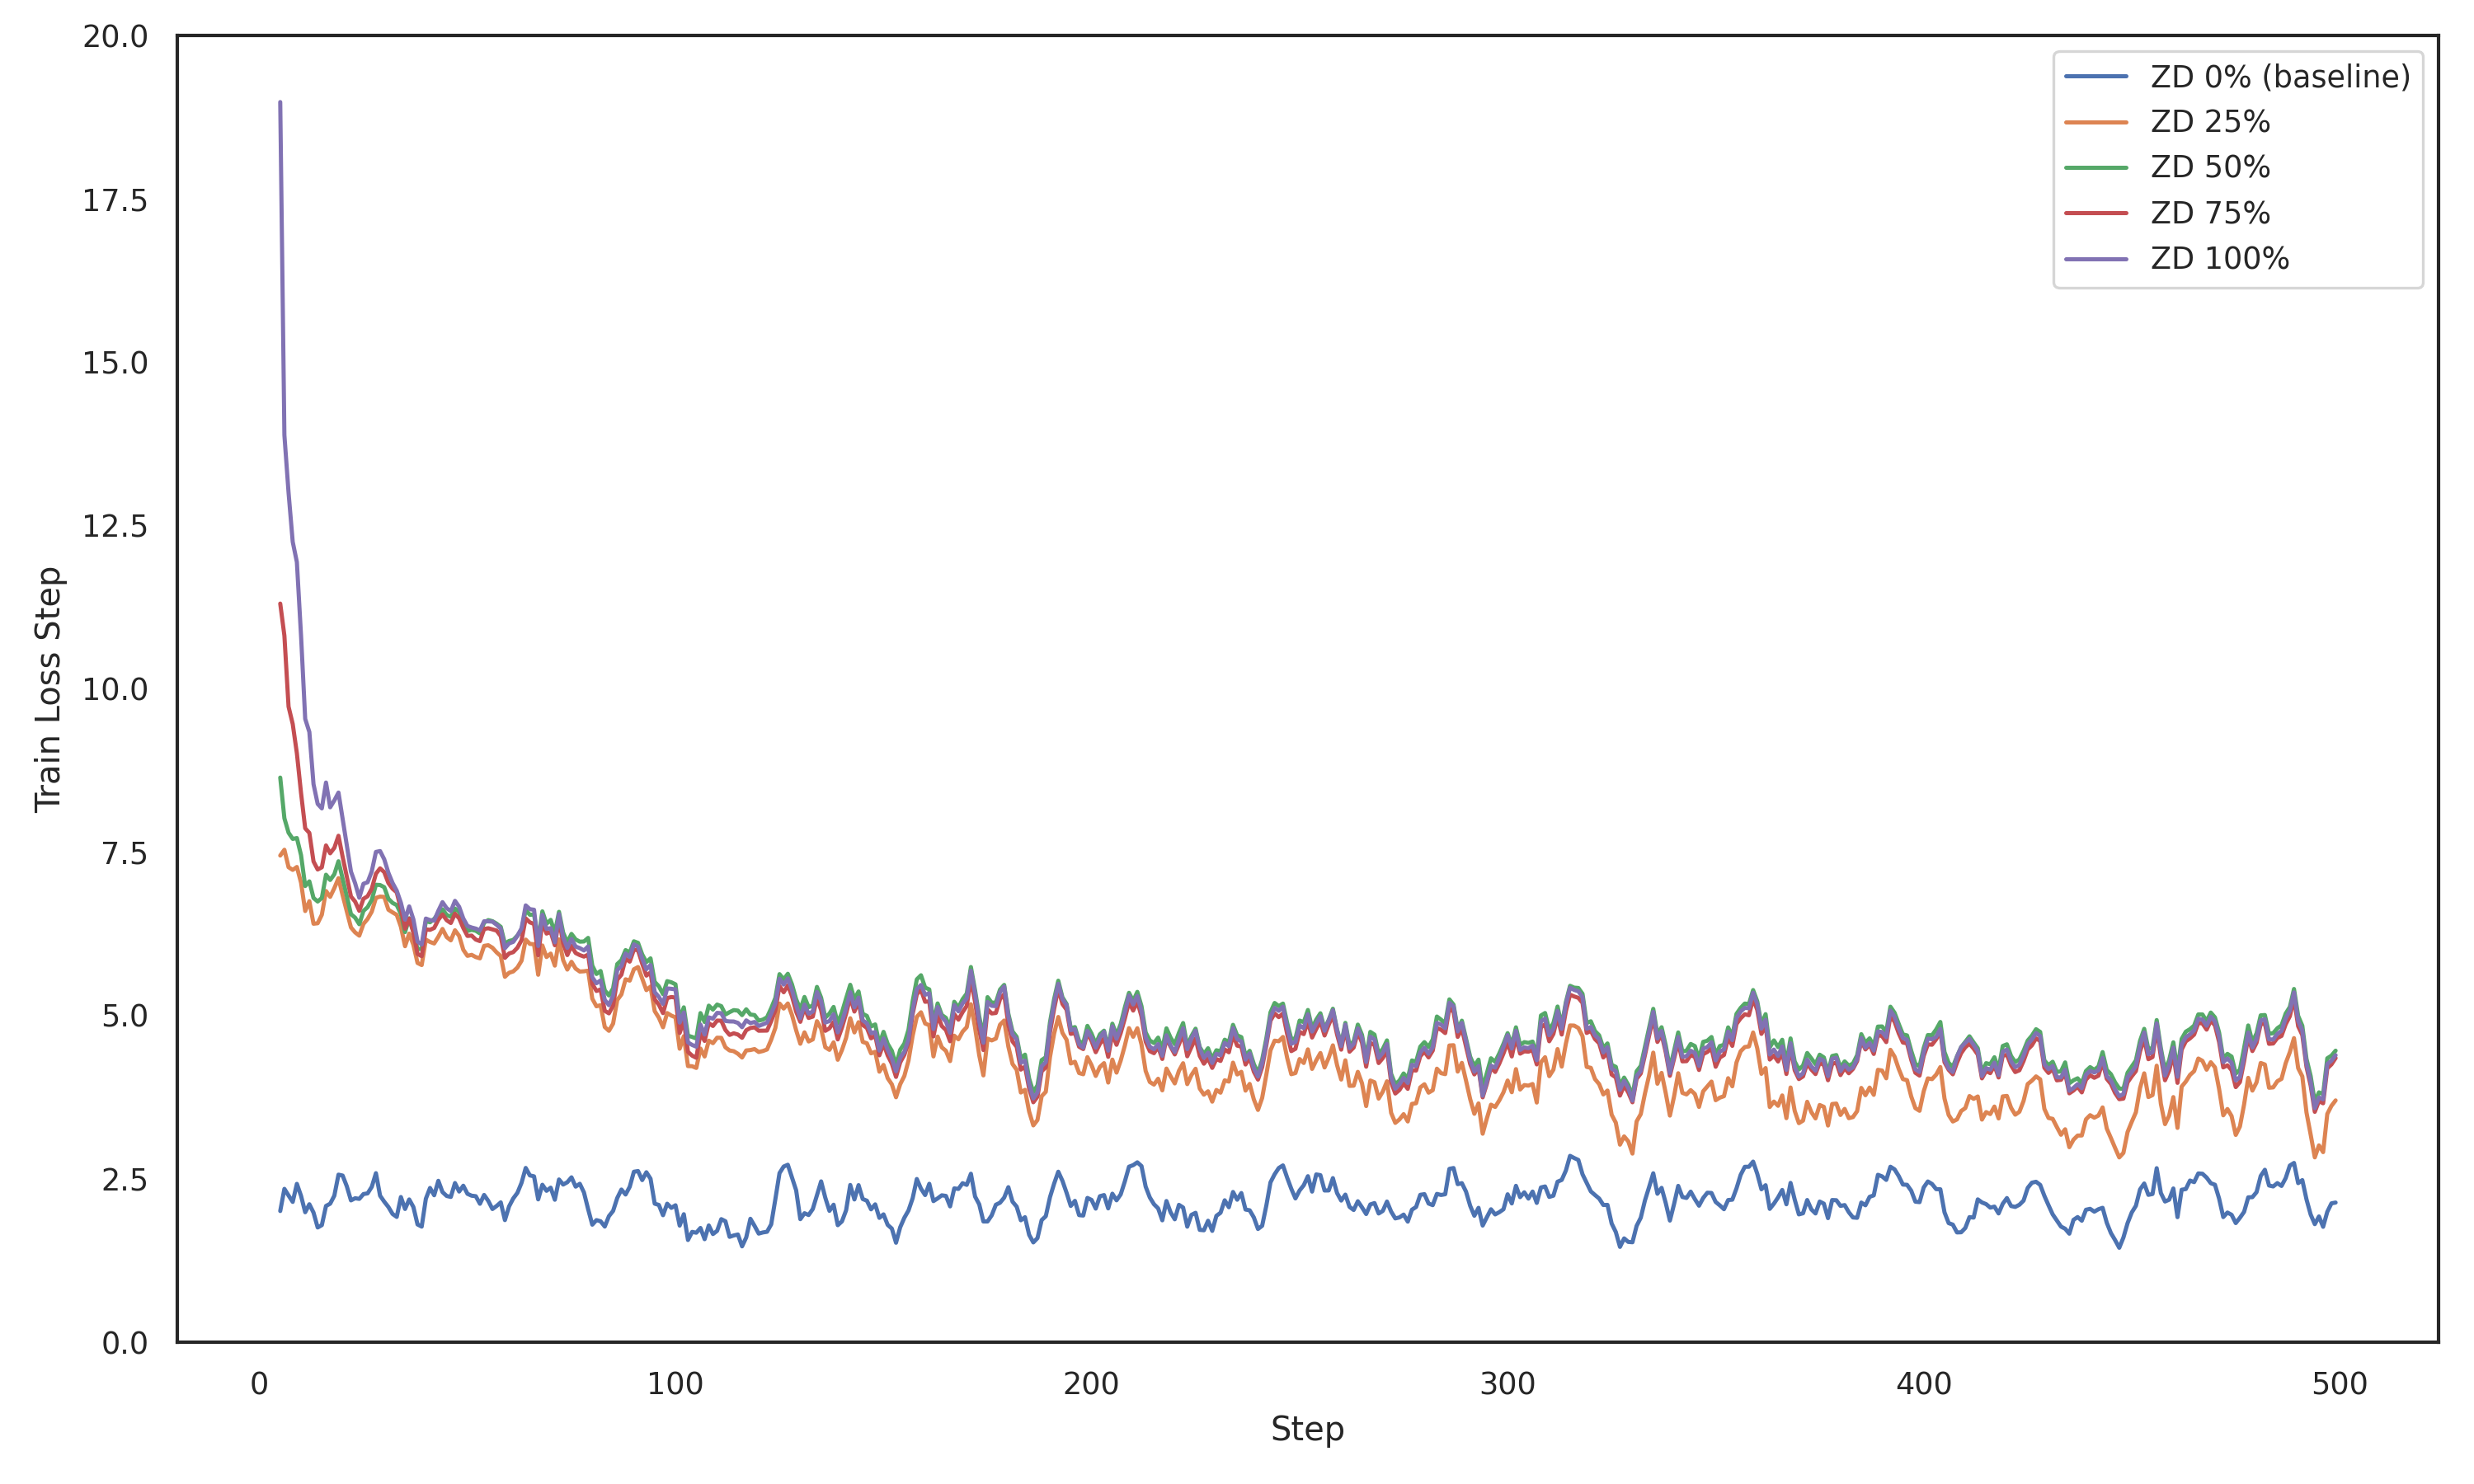
\includegraphics[width=\linewidth]{../data/plots/ZD_least_important.png}
    \caption{ZD}
  \end{subfigure}
  \hfill
  \begin{subfigure}[b]{0.45\textwidth}
    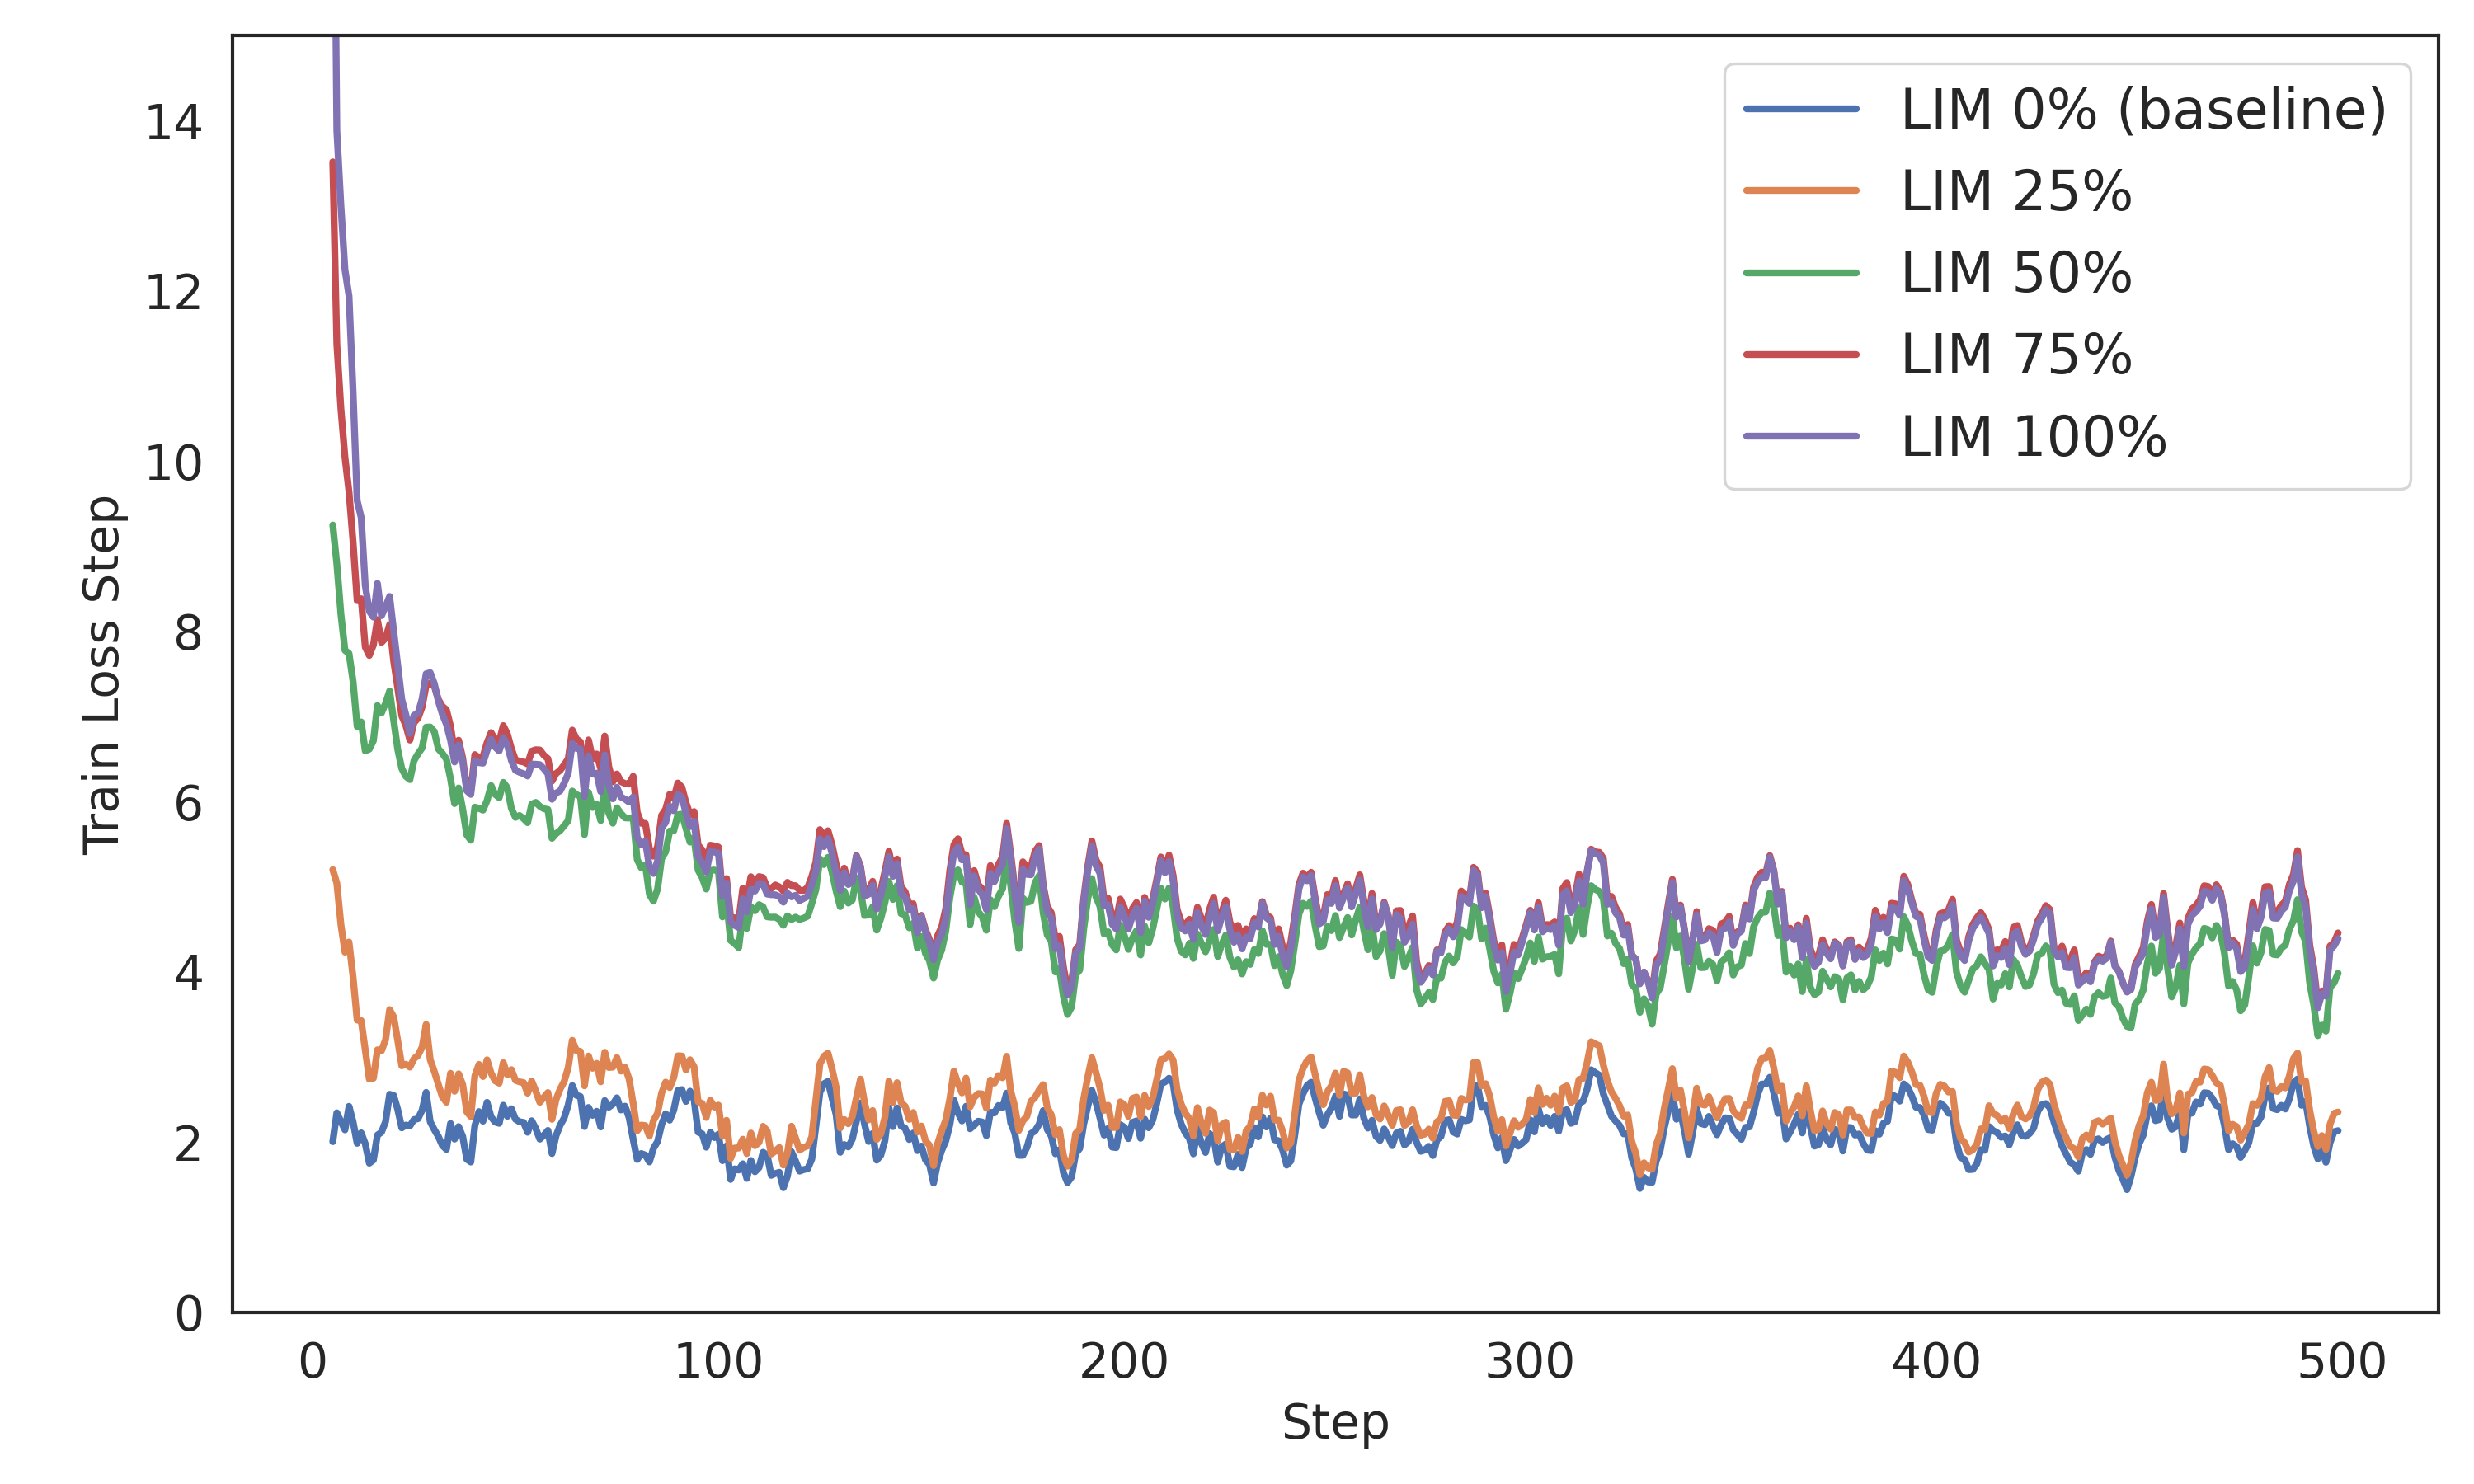
\includegraphics[width=\linewidth]{../data/plots/LIM_most_important.png}
    \caption{LIM}
  \end{subfigure}
  \vspace{0.5em}
  \caption{Plot \textbf{a} shows how quantizing \(n\%\) of the least important layers influences the loss. Plot \textbf{b} shows how quantizing \(n\%\) of the most important layers influences the loss. In case of ZD, quantizing as little as 10\% of least important layers produces model significantly worse than the baseline.
  }
  \label{fig:layers}
\end{figure}

Thus we decide to quantize only \(25\%\) most important layers according to LIM score, so we can compare our distilled models on some of the common benchmarks.

In our experiments we will focus on the comparison of 3 aspects:

\begin{itemize}
    \item how quantization (1b or 1.58) influences the model training;
    \item how BitLinear architecture influences the model training;
    \item how the loss function influences the model training.
\end{itemize}



\begin{table}[ht]
  \centering
  \begin{tabular}{ccccccc}
    \toprule
    Quantization & Model & Loss & HellaSwag (\%) & MathQA (\%)  & Winogrande (\%) & WikiText (Perpl.) \\
    \midrule
    1-bit & BitNet & CE & 30.0 & 22.9 & 50.3 & 268.0 \\
    1.58-bit & BitNet & CE & 30.9 & 22.8 & 51.5 & 255.0 \\
    1.58-bit & FBI & CE& 30.3 & 22.2 & \textbf{53.2} & 278.3 \\
    1.58-bit & OneBit &  CE & \textbf{31.1} & 23.1 & 51.0 & 235.8 \\
    1.58-bit & OneBit & KL & 30.9 & \textbf{23.6} & 51.7 & 237.7 \\
    1.58-bit & OneBit & CAKL & 30.8 & 23.0 & 50.8 & \textbf{233.7} \\
    1.58-bit & OneBit & WD & 25.6 & 20.9 & 50.4 & 780769.3 \\
    \midrule
    &Teacher && 35.0 & 23.2 & 56.8  & 24.1 \\ 
    \bottomrule
  \end{tabular}
  \vspace{0.5em}
  \caption{Model performance on the chosen benchmarks}
  \label{table:bchmrk}
\end{table}


To evaluate our models, we will use EleutherAI's evaluation suite \cite{eval-harness}, which provides a set of benchmarks for LLMs. We will focus on the accuracy of three common LLM evaluation tasks: HellaSwag \cite{zellers2019hellaswag}, MathQA \cite{amini2019mathqa} and Winogrande \cite{sakaguchi2019winogrande}. In addition to these, we benchmarked our models with perplexity on the WikiText dataset \cite{merity2016pointer}. All of the results are presented in Table \ref{table:bchmrk}.

\subsection{Comparison with the teacher}
Compared to modern LLMs, the teacher achieves low scores on the three presented benchmarks. Nevertheless, it can still serve as a reference and tell us how far we were from distilling models into quantized versions. Tracher wins all of three benchmarks, but on MathQA gives similar accuracy to most of the models. It is probably due because, SmolLM2 135M Instruct does not understand mathematics itself very well. Still, we wanted to benchmark our models on at least one mathematics-oriented task, as most of our text was from the hard sciences domain.

Saying all that, the teacher model differs a lot from the distilled models on a perplexity metric. The text generated by the teacher is still much more coherent than that generated by the distilled models. We suspect this is because the teacher was trained on a much larger corpus. We believe that with bigger computational resources and longer training, most of our models could achieve much better performance.

\subsection{Quantization precision}
Two quantization precisions (1-bit and 1.58-bit) were investigated. For both models, we used the Cross-Entropy loss function and BitNet model for the quantization. Benchmarks for both configurations are presented in the first two rows of Table \ref{table:bchmrk}. While both achieve similar results on the second benchmark, 1.58-bit quantization outperforms 1-bit in the first and the third benchmark. 1.58-bit precision model also achieves visibly lower perplexity. In the Figure \ref{fig:quant}, one can see training loss functions and fit-flip ratios for the two quantization precisions. The training losses of the two methods are very similar, although 1.58-bit seems to be shifted slightly lower. On the other hand, their flip-flop ratios seem to differ greatly. 1-bit precision is characterized by a more unstable and overall greater flip-flop ratio. We can conclude, that the increased precision helps the model's performance, which is an anticipated result. Although it is hard to find clear instabilities in the training loss of 1-bit model, the bigger instability of the quantized layers results in a worse performance on all of the analyzed benchmarks.

\begin{figure}[ht]
  \centering
  \begin{subfigure}[b]{0.45\textwidth}
    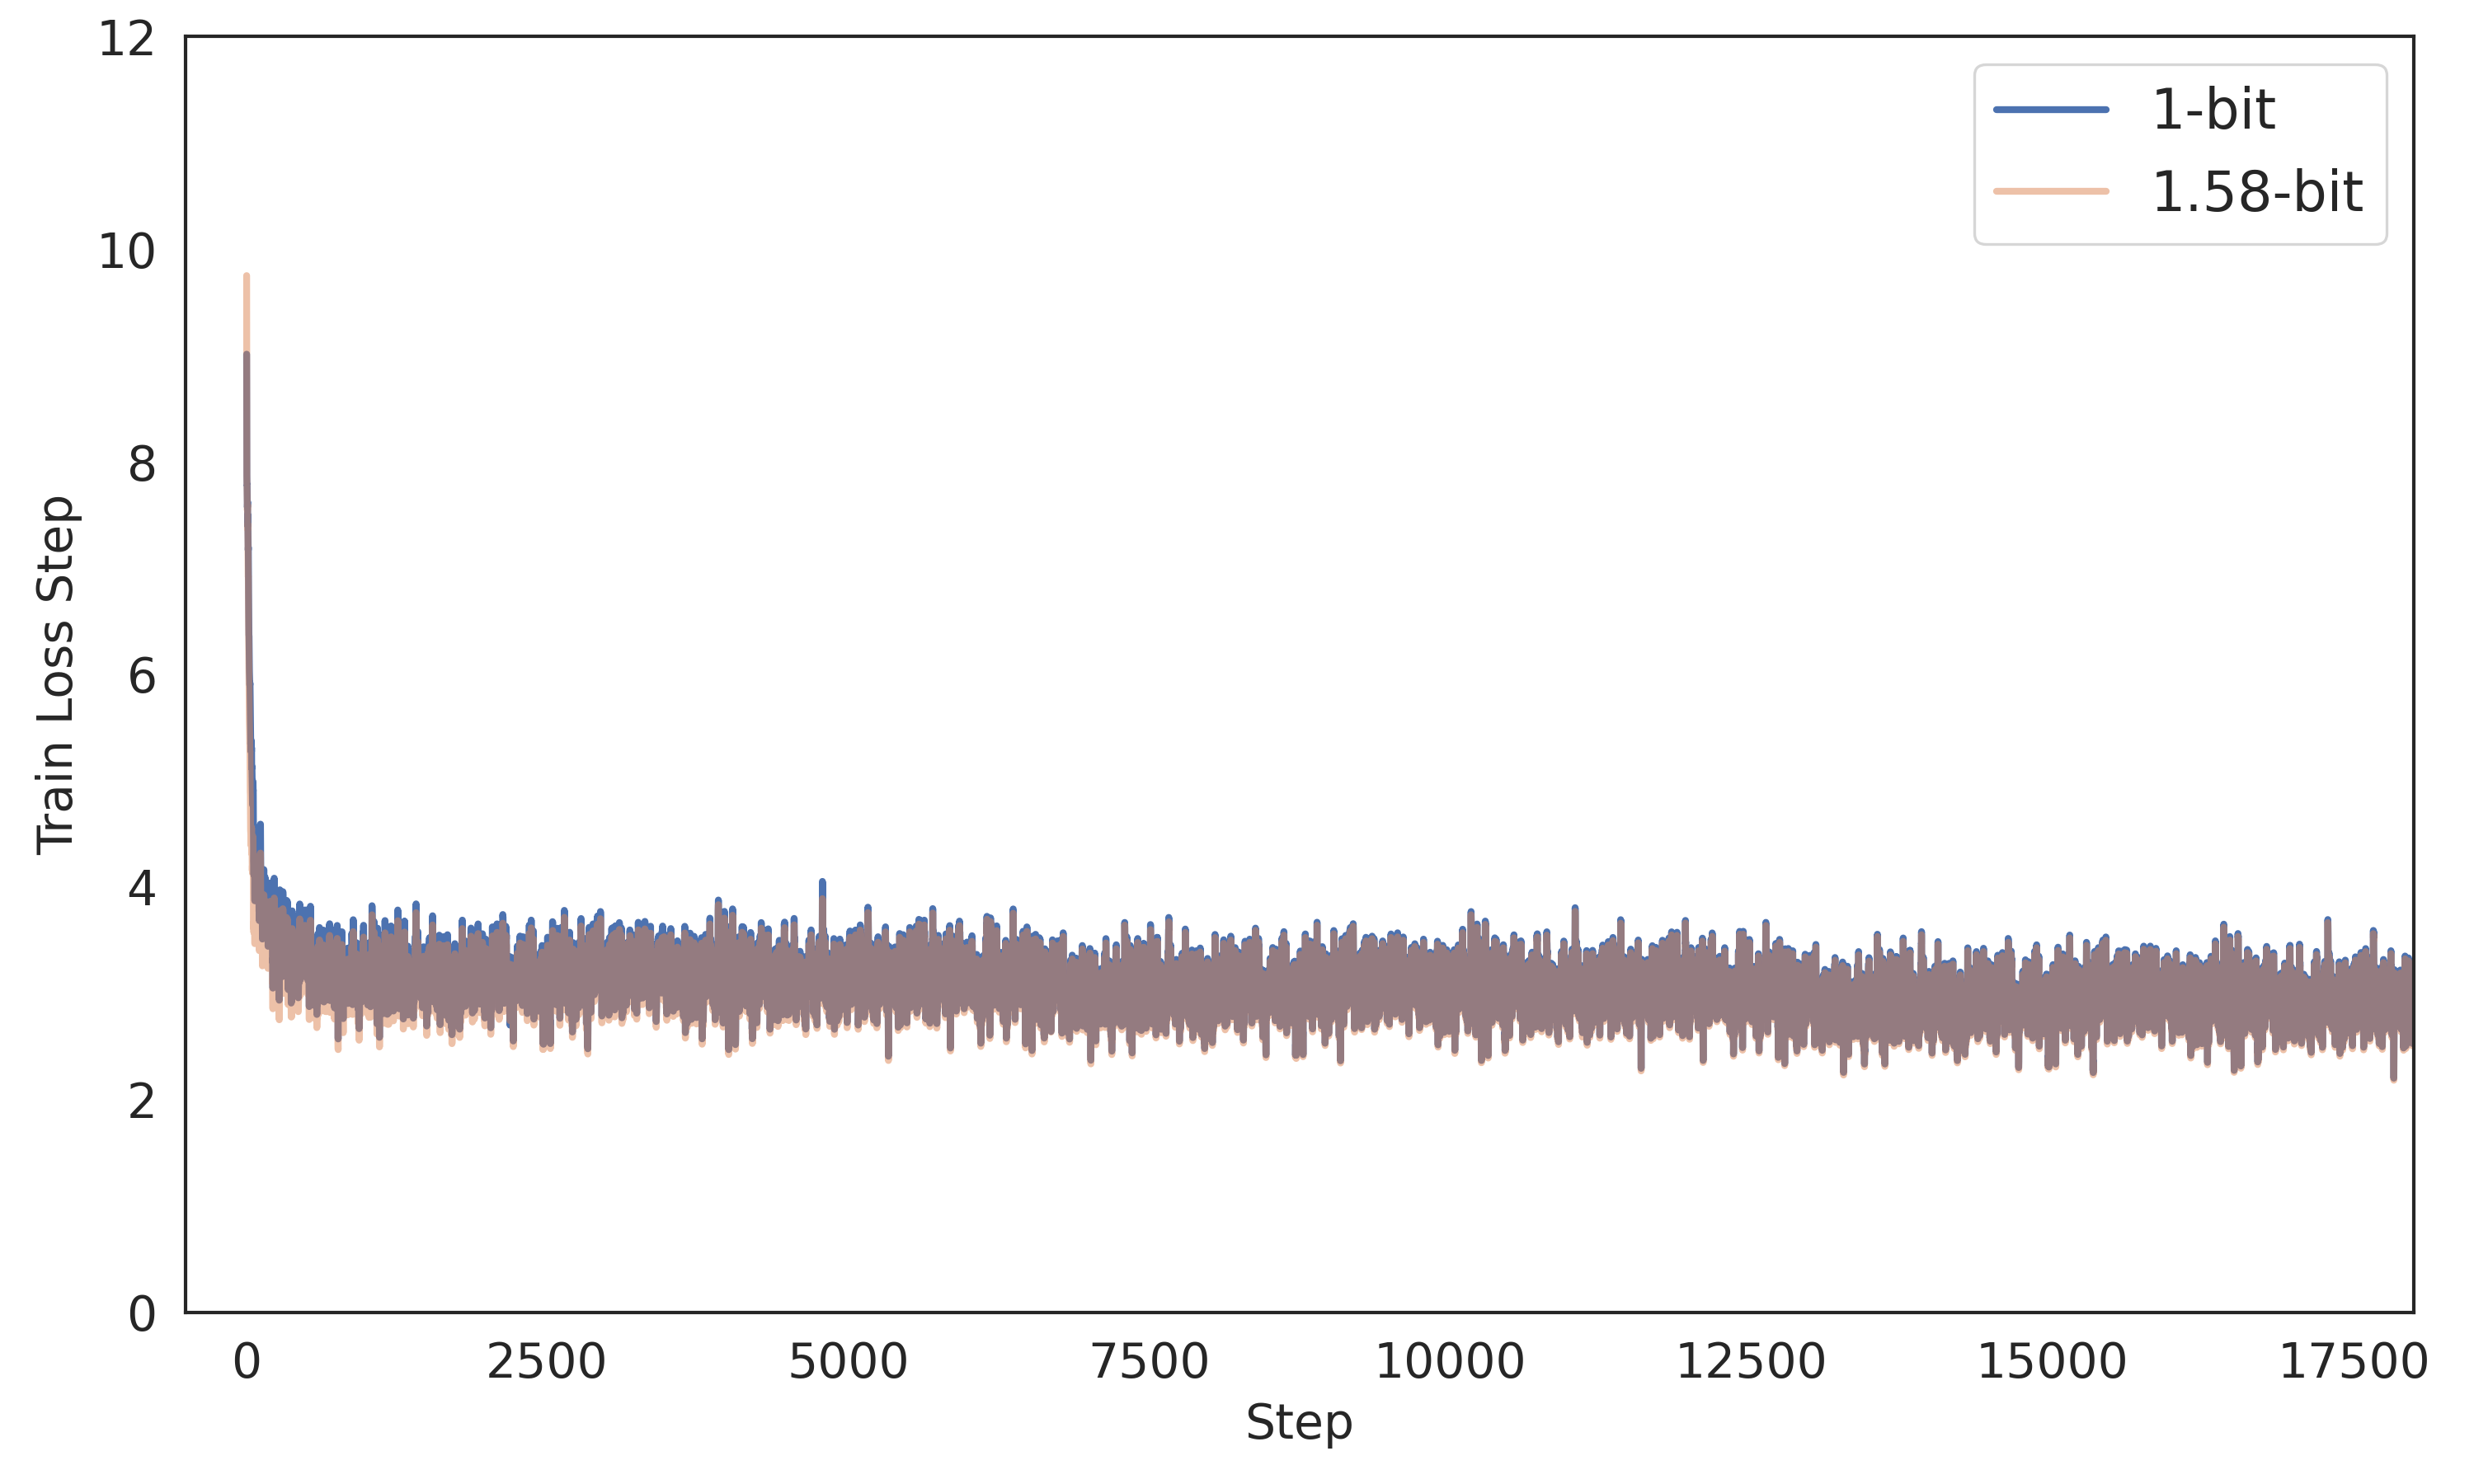
\includegraphics[width=\linewidth]{../data/plots/quant_precision.png}
    \caption{Training Loss}
  \end{subfigure}
  \hfill
  \begin{subfigure}[b]{0.45\textwidth}
    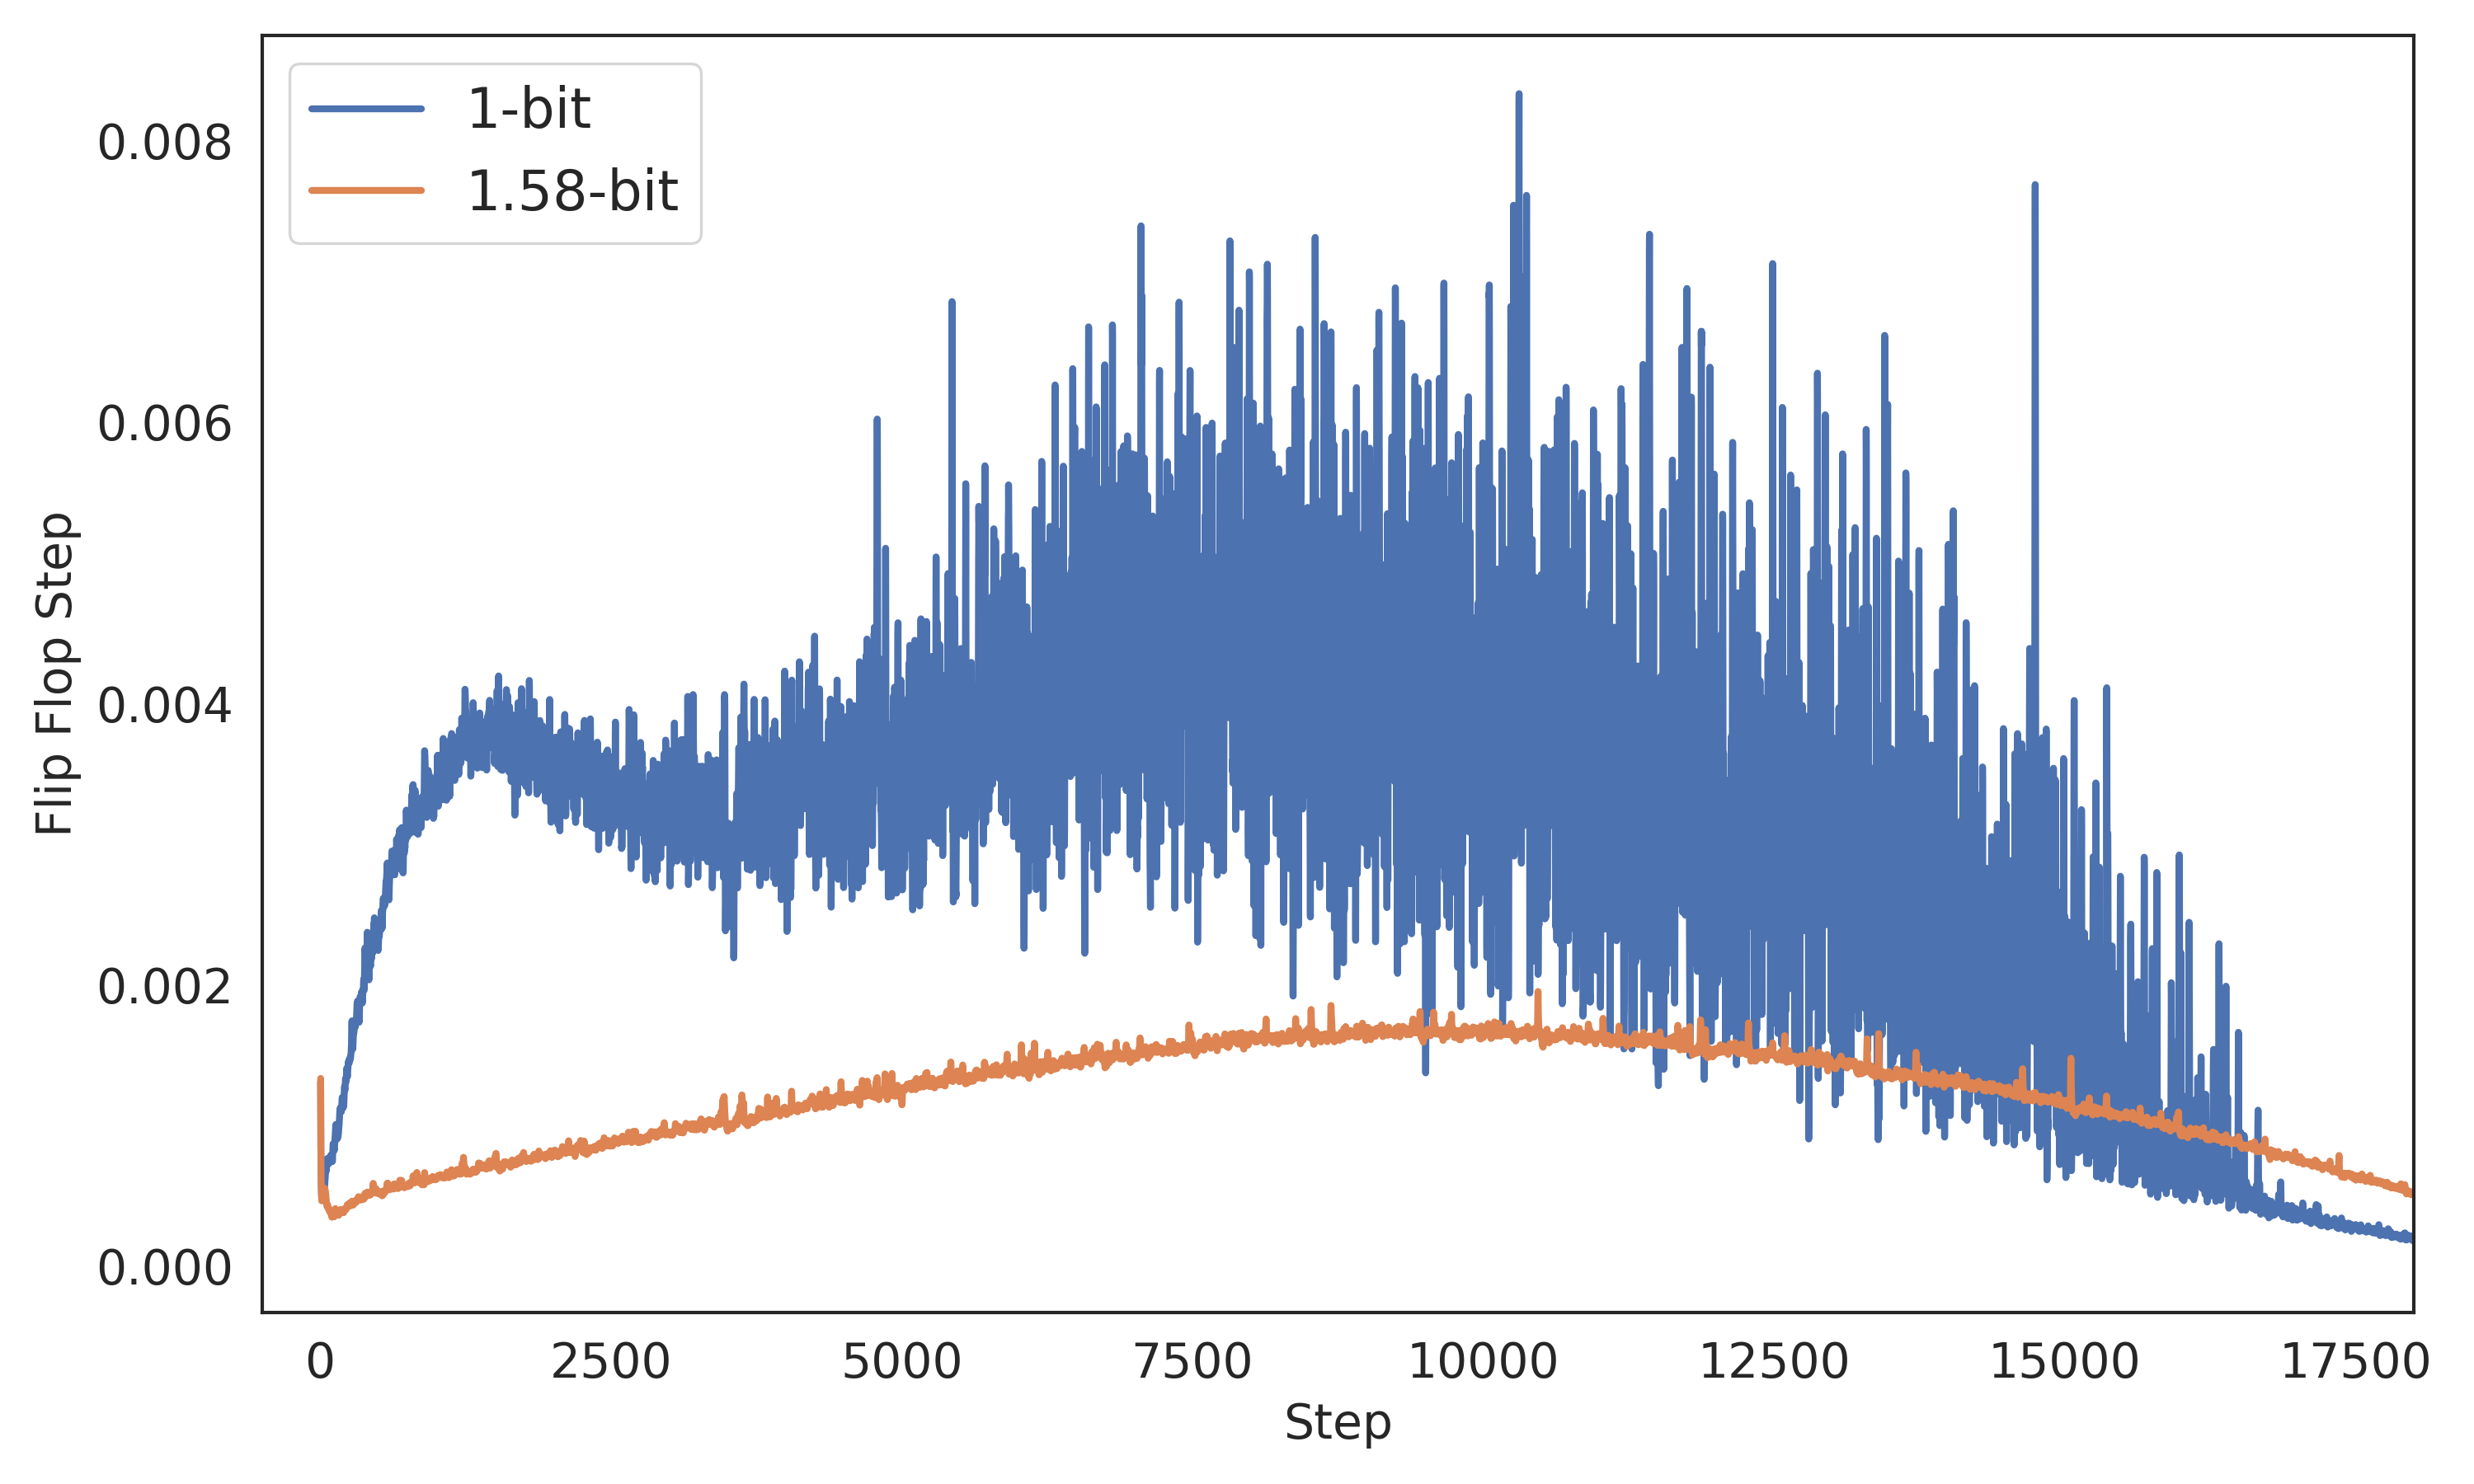
\includegraphics[width=\linewidth]{../data/plots/quant_precision_ff.png}
    \caption{Flip-Flop Ratio}
  \end{subfigure}
  \caption{Plot of the training losses for the two quantization precisions and flip-flop ratio. Training loss plots strongly overlap, but one can see that 1-bit precision gave slightly bigger losses throughout the training.}
  \label{fig:quant}
\end{figure}

\subsection{Quantization method}
One of the aims of the following work was to check how the distilled model's performance changes subject to a change in the quantization method. Rows \(2-4\) of Table \ref{table:bchmrk} correspond to this comparison. All models were tested using 1.58-bit quantization. Cross-entropy served as a loss function. OneBit seems to outperform the two other methods in both benchmarks, achieving the best accuracy on HellaSwag among all of the tested configurations. It also achieves the lowest perplexity among the three different quantization methods. FBI method wins benchmark on Winograde task. In the Figure \ref{fig:bitlin}, one can see the training losses and flip-flop ratios for OneBit, FBI, and BitNet. While training losses of all methods have a similar mean, they differ a lot in variance. Surprisingly, OneBit has the highest training loss variance, while FBI has the lowest. Flip-flop ratios of BitNet and OneBit appear to be very similar through the training, while FBI has a substantially larger average flip-flop ratio, which does not seem to decrease in later steps of the training, unlike what happens in the previous two methods. OneBit seems to give the best results on the benchmarks. It was anticipated that BitNet would perform worse as it does not use additional trainable weights in quantized modules. FBI has such parameters, but we can see that it suffers from quantized layers' instability, which could be the cause of the worse final performance.

\begin{figure}[ht]
  \centering
  \begin{subfigure}[b]{0.45\textwidth}
    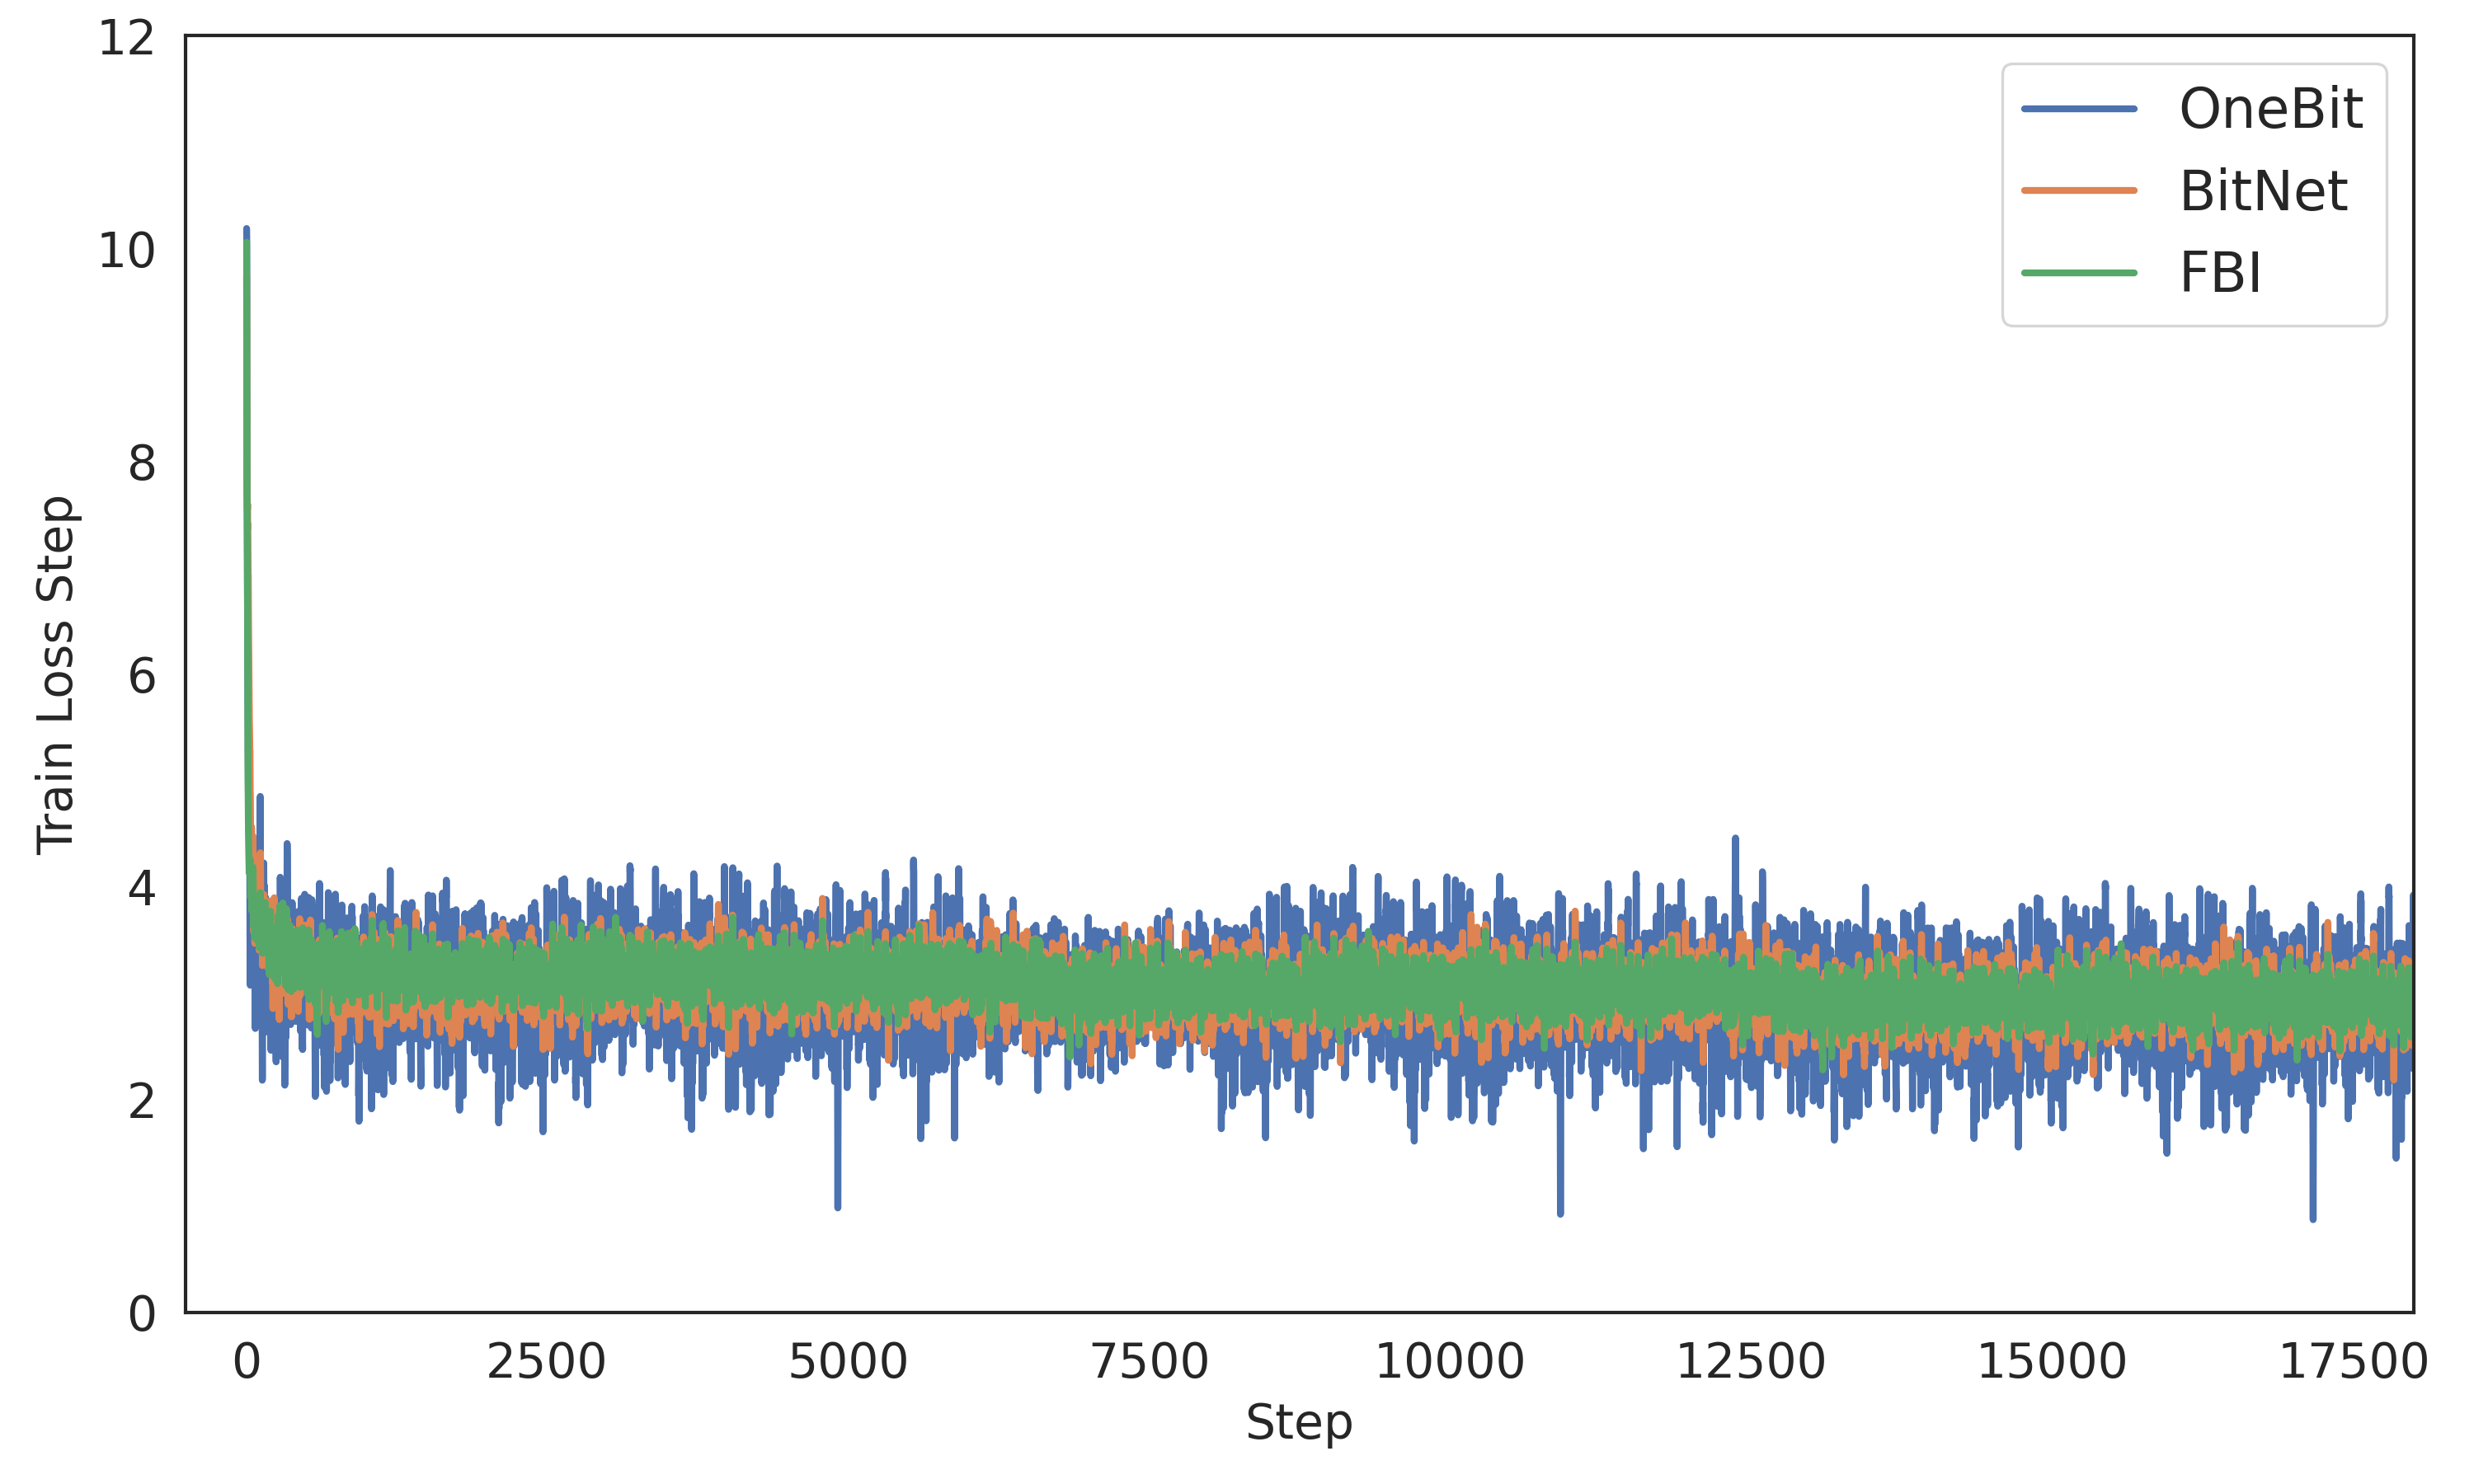
\includegraphics[width=\linewidth]{../data/plots/quant_layer.png}
    \caption{Training Loss}
  \end{subfigure}
  \hfill
  \begin{subfigure}[b]{0.45\textwidth}
    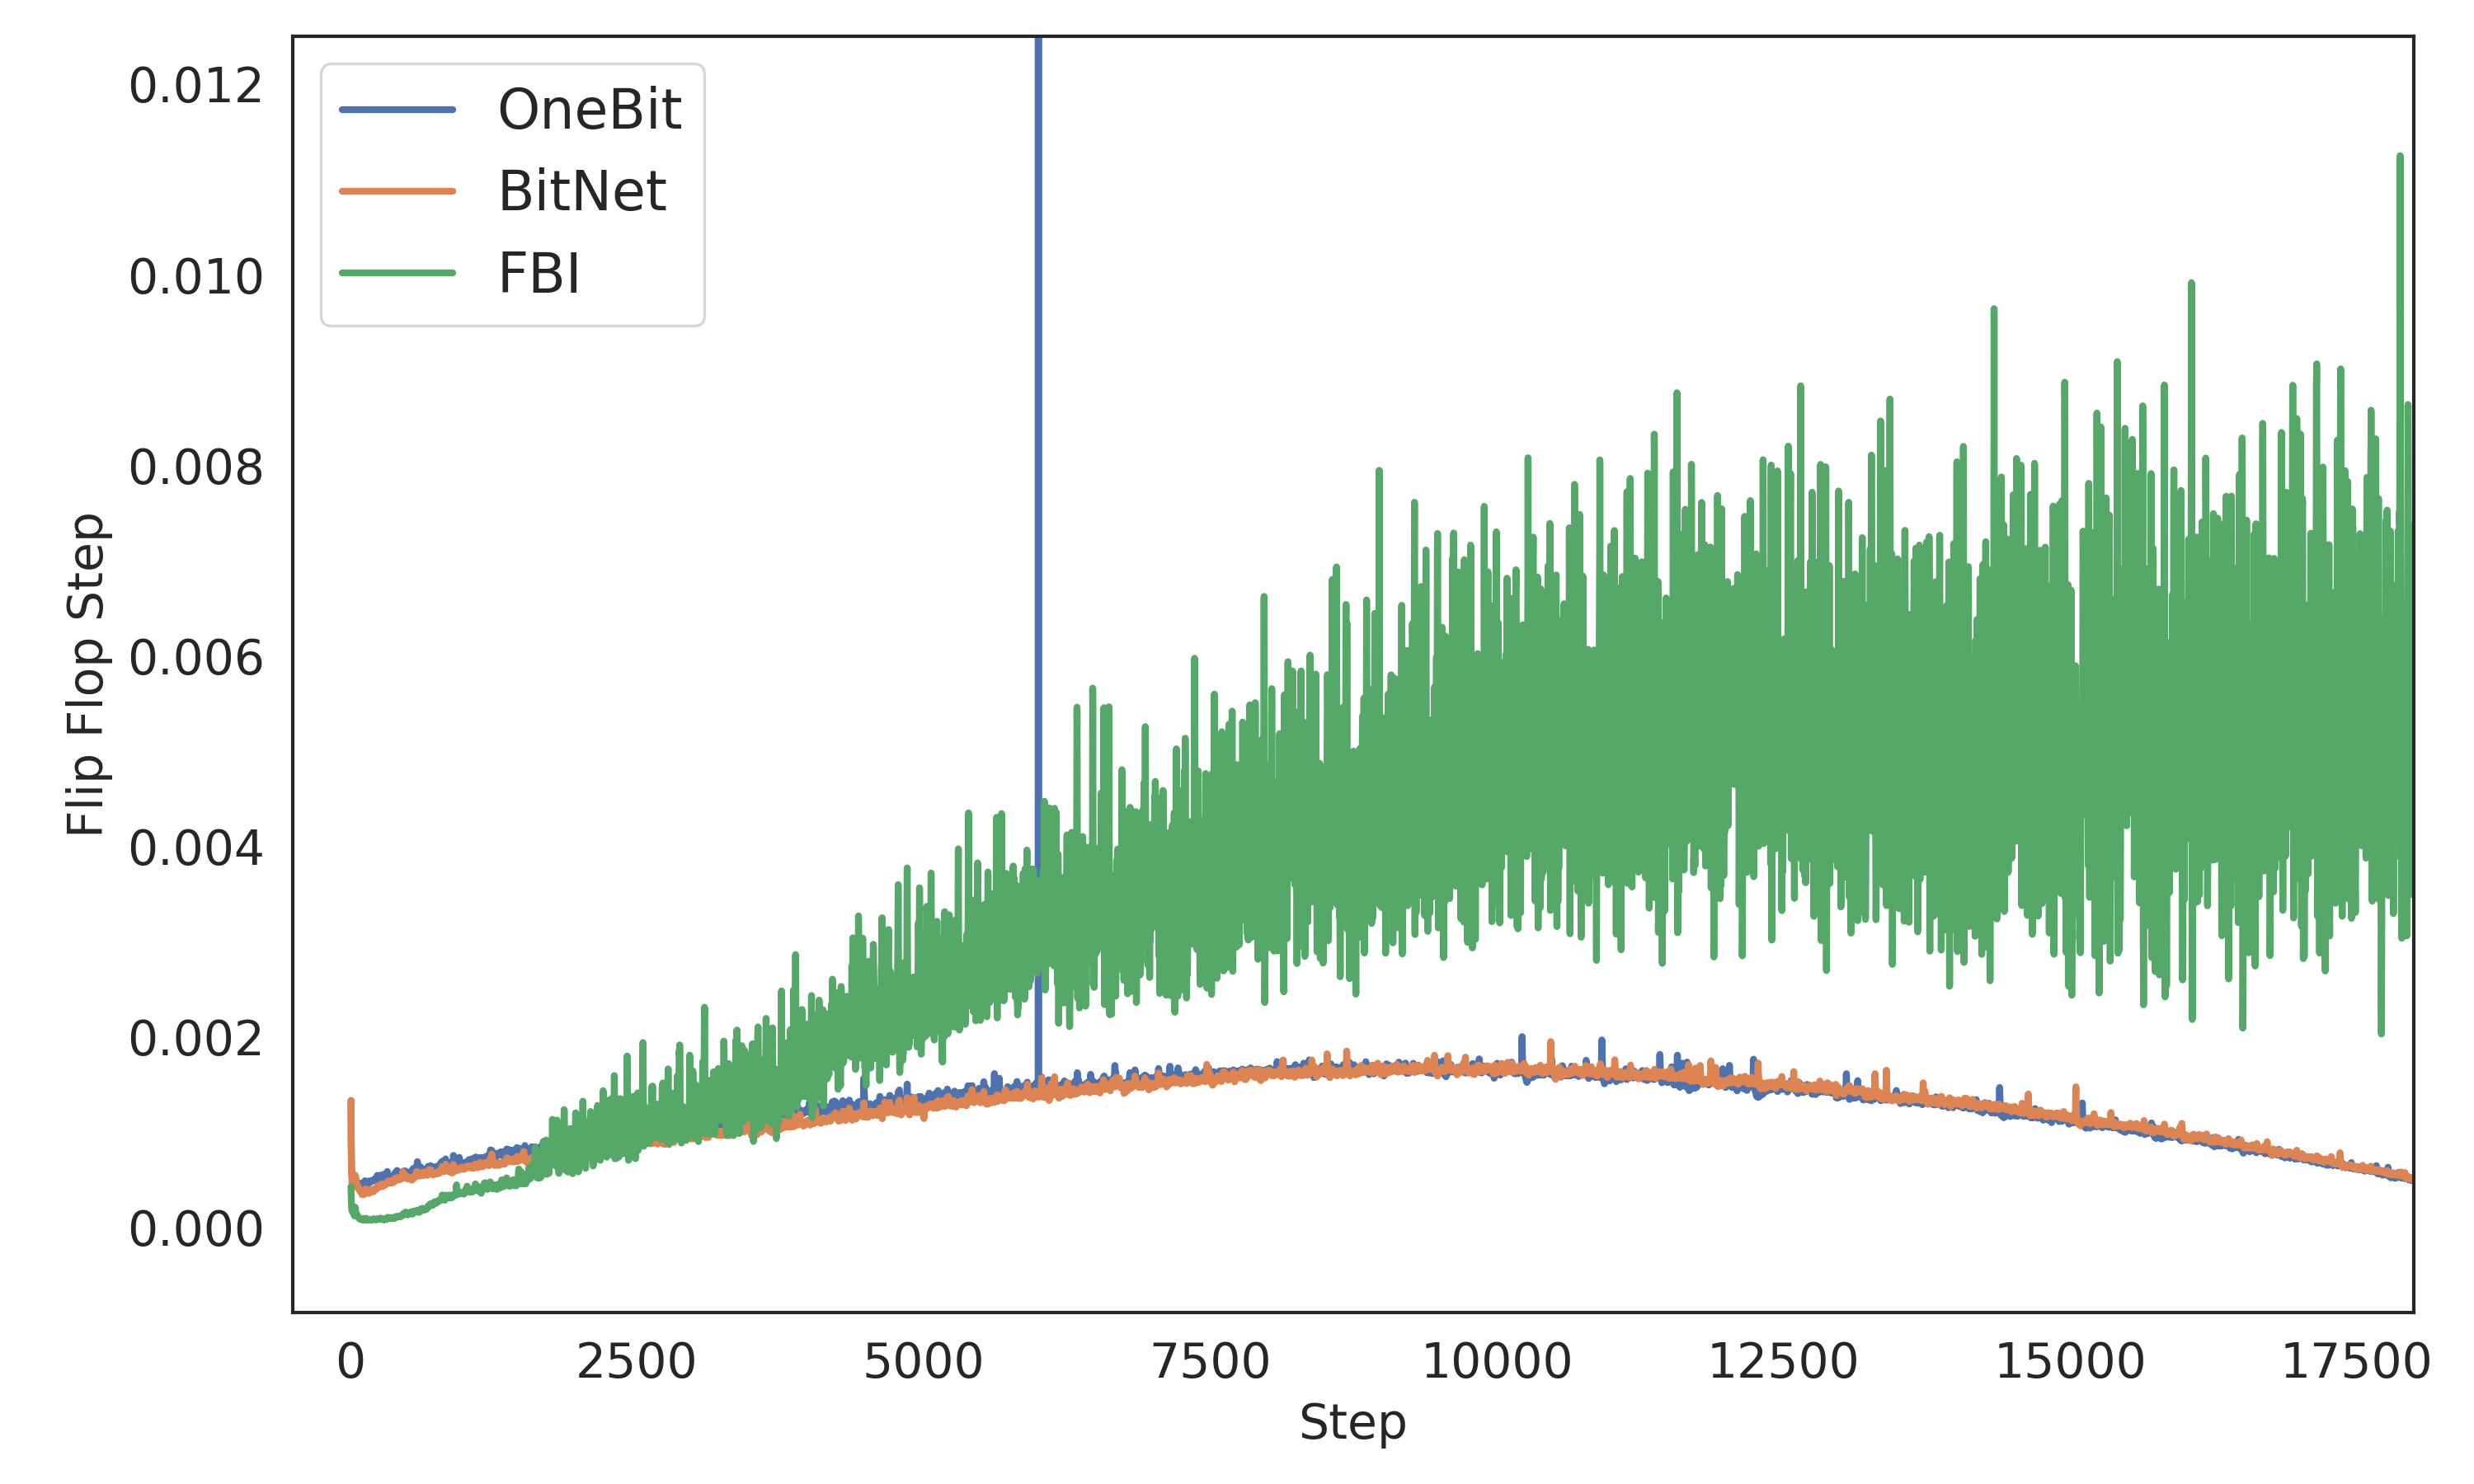
\includegraphics[width=\linewidth]{../data/plots/quant_layer_ff.png}
    \caption{Flip-Flop Ratio}
  \end{subfigure}
  \caption{Plot of the training losses for the three quantization methods and their flip-flop ratios.}
  \label{fig:bitlin}
\end{figure}

\subsection{Loss Function}
At last, we compare how the loss function influences the performance of the distilled model. We investigated four loss functions defined above (Cross-Entropy, KL, Confidence-Aware KL, and Wasserstein Distance). All models in this comparison were quantized using OneBit with 1.58-bit precision. Their benchmark performance was shown in the last four rows of Table \ref{table:bchmrk}. Among the models, the one using Cross-Entropy performs the best on the HellSwag benchmark, and the one using KL divergence wins the MathQA and Winogrande. The lowest perplexity is achieved by the model using CAKL. The model using the Wasserstein distance diverges strongly from all other models on all metrics. Its HellaSwag performance is close to the model choosing its answers at random. Its perplexity is hundreds of times higher than other models', which indicates that the model did not converge at all. We checked that usually, the model outputs a random key or does not output anything. It can be caused by either a bug in the Wasserstein loss implementation or by the fact that our implementation of the Wasserstein Distance compares mass probabilities in sorted order, without taking into account the alignment between token identities, which may distort the learning signal and prevent meaningful gradient flow during distillation. This comparison does not have a clear winning method, but we can see that using Cross-Entropy, KL Divergence, and CAKL can be reliable choices during distillation. In the Figure \ref{fig:loss}, we can see training losses for different models among flip-flop ratios. The plots of the training loss curves were separated as different losses operate on different scales, and it is hard to compare them nominally. First three losses drop rapidly and slowly decrease throughout training afterwards. Wasserstein distance loss curve falls drastically around \(4000\) step, but it could be a result of changing data distribution. Cross-Entropy, KL, and CAKL models have very similar flip-flop ratio curves following a quadratic-like pattern, common in our experiments.

\begin{figure}[ht]
  \centering
  \begin{subfigure}[b]{0.45\textwidth}
    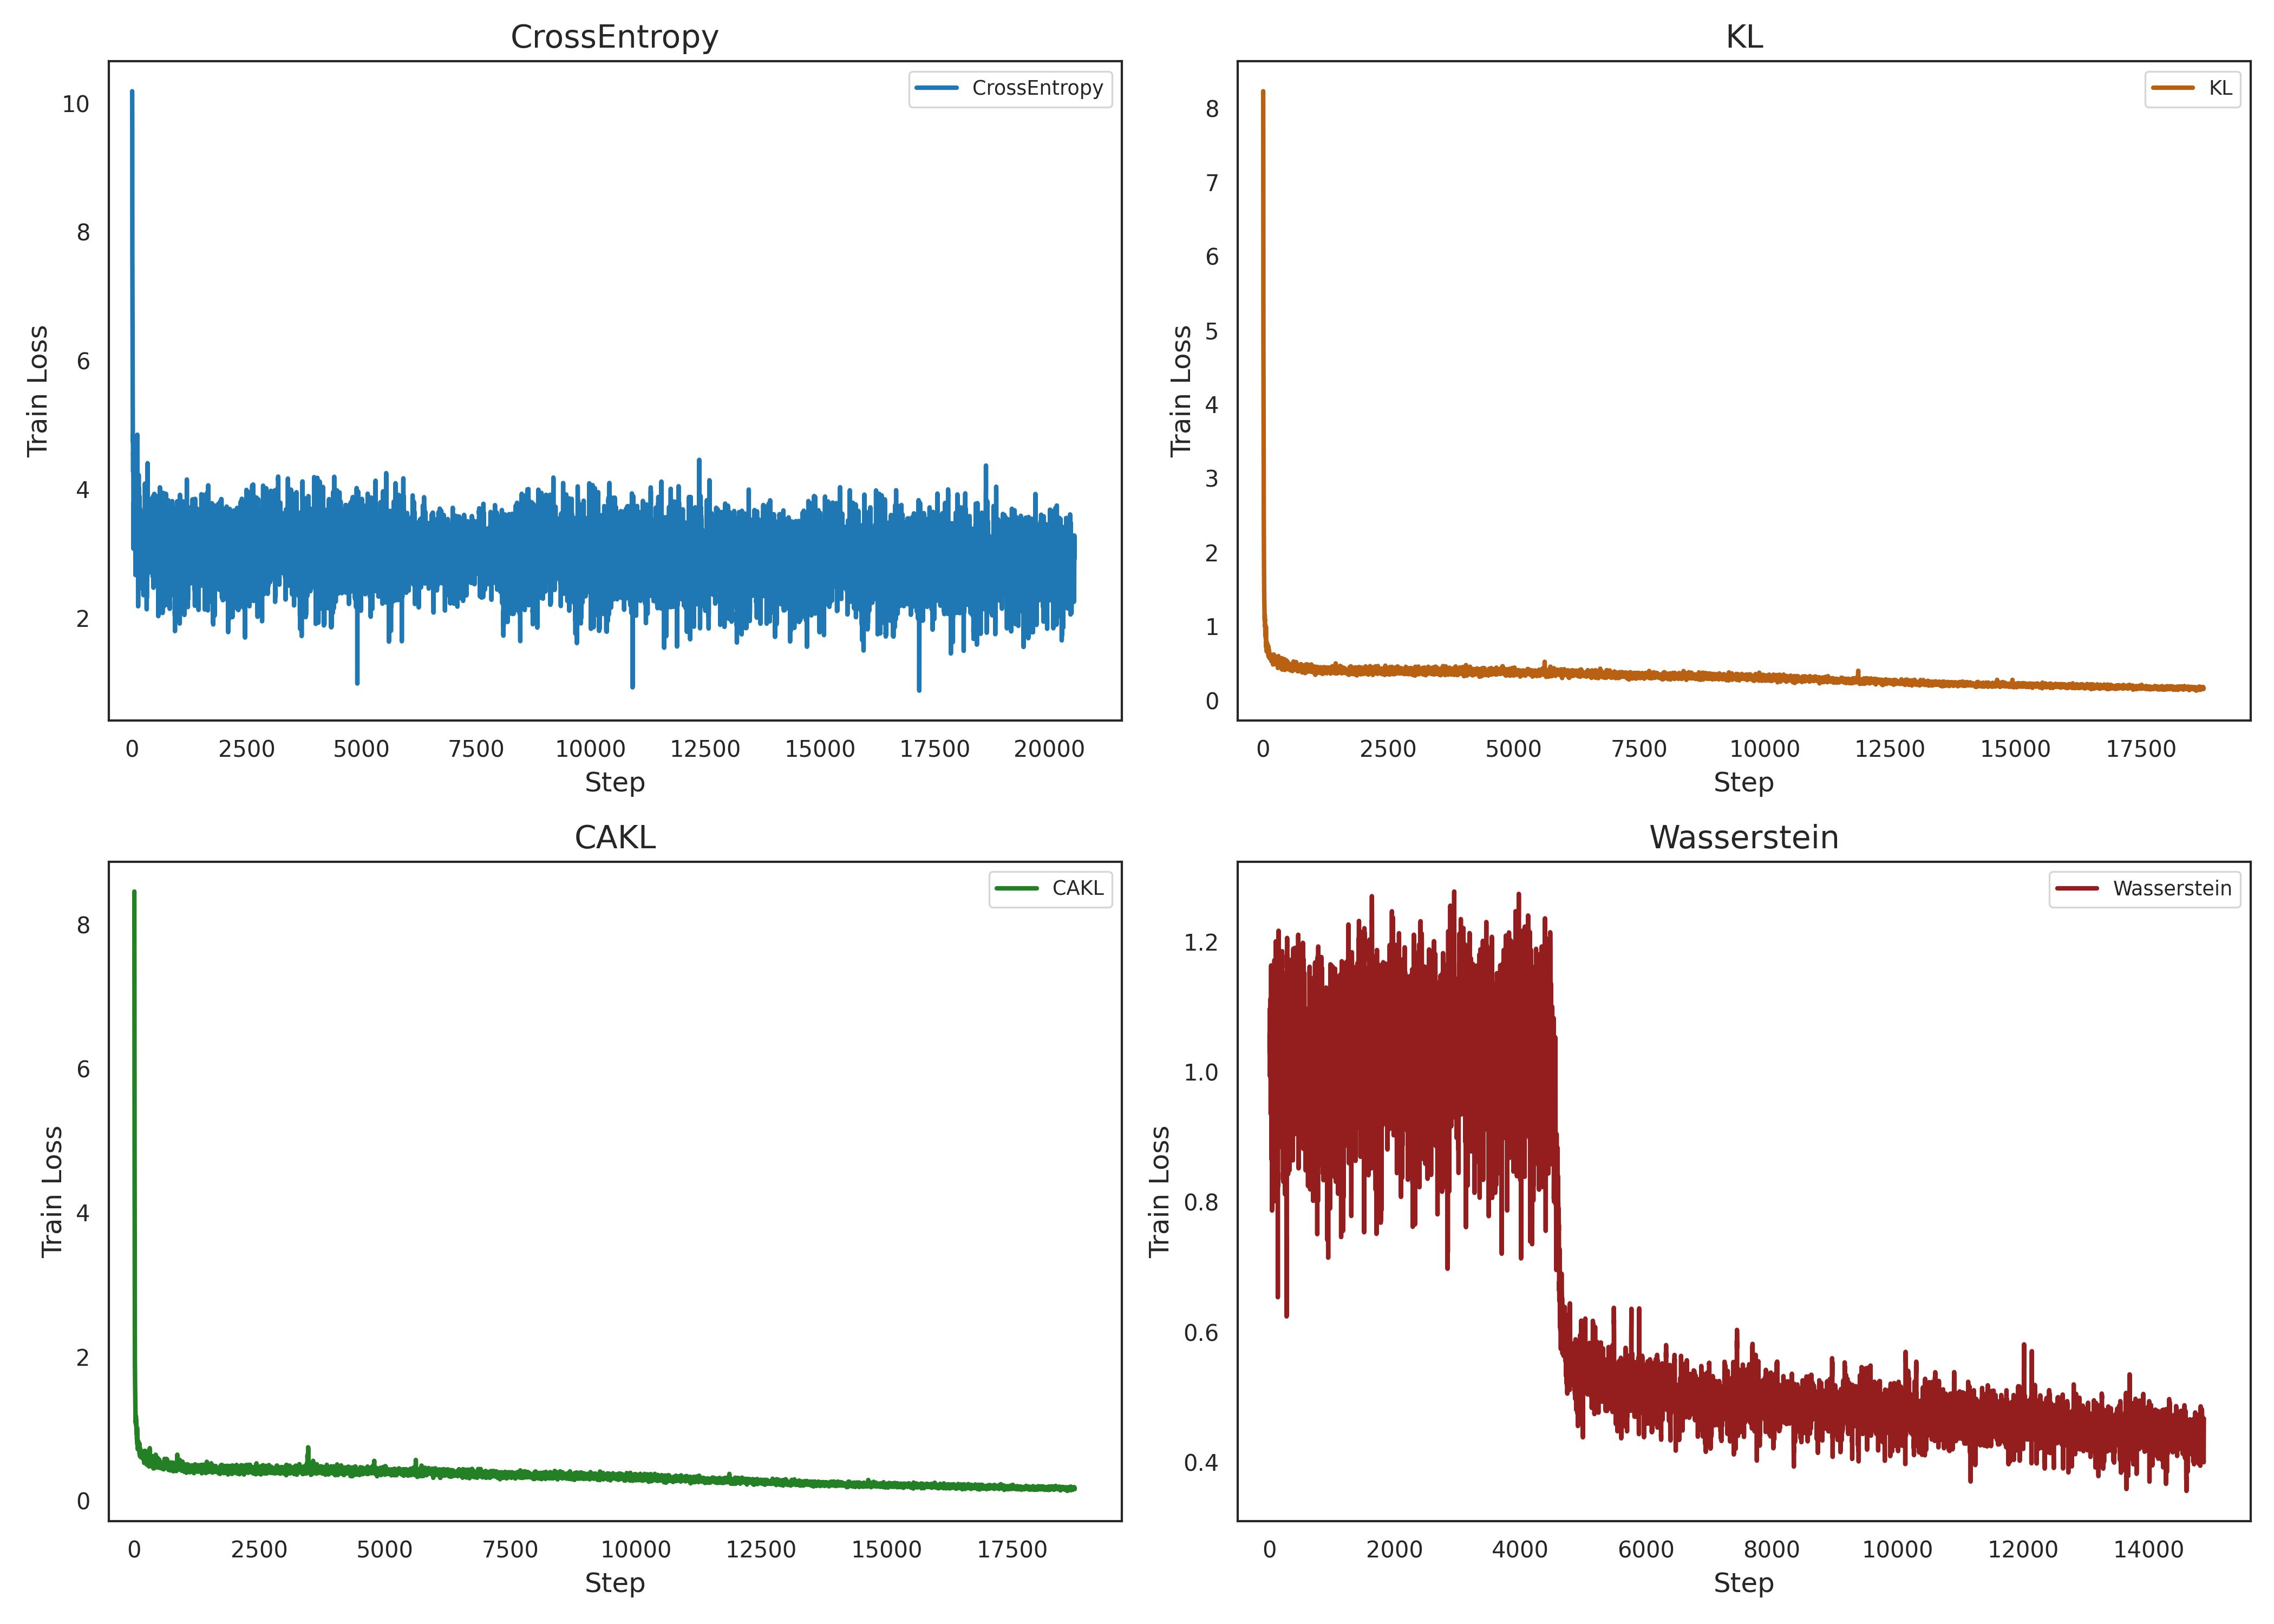
\includegraphics[width=\linewidth]{../data/plots/loss_comparison_grid.png}
    \caption{Training Losses}
  \end{subfigure}
  \hfill
  \begin{subfigure}[b]{0.45\textwidth}
    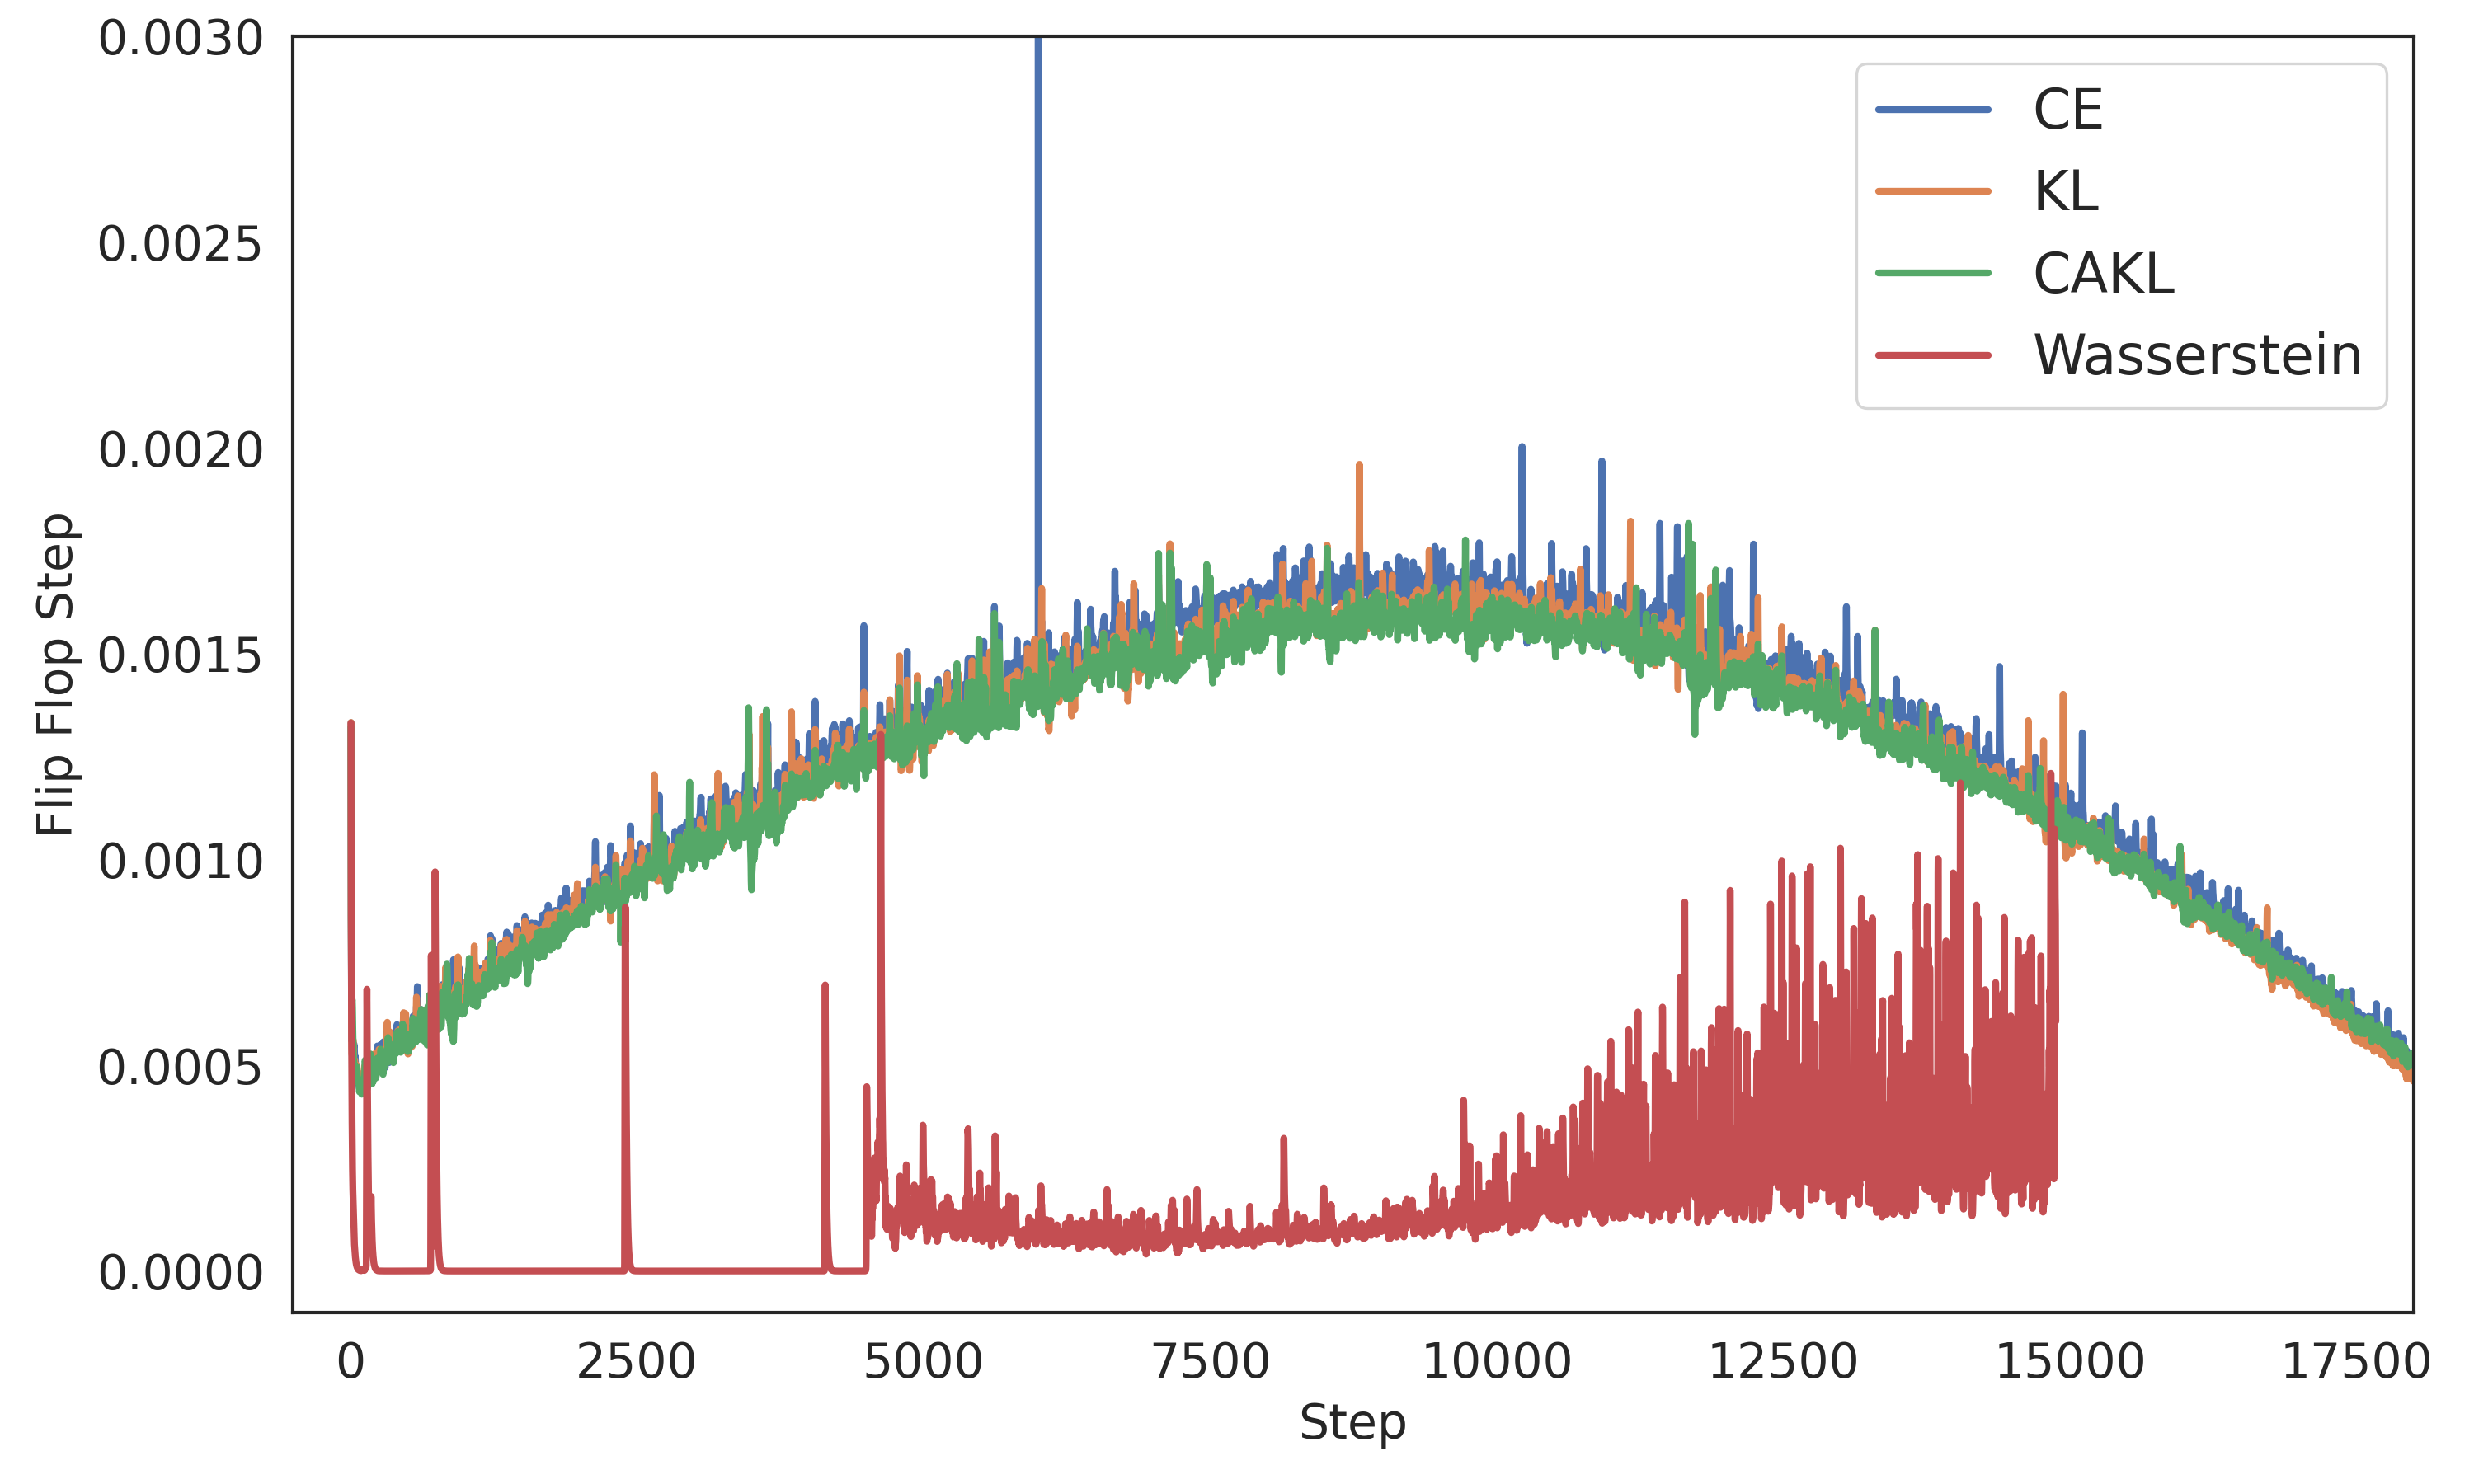
\includegraphics[width=\linewidth]{../data/plots/quant_loss_ff.png}
    \caption{Flip-Flop Ratio}
  \end{subfigure}
  \caption{Plots of the training losses and flip-flop ratio for the four loss functions. As training losses are different here, they were put in separate plots.}
  \label{fig:loss}
\end{figure}

\section{Conclusion and future work}
Our work aimed to compare and investigate existing methods of Large Language Models quantization to 1.58-bit precision through distillation. We reviewed how distillation performance depends on a used loss function and quantization methods. We additionally checked that increasing precision from 1-bit truly affects the model's performance, giving a better performance on benchmarks. Our experiments show that among the three quantization models (OneBit, BitNet, and FBI), OneBit gives the best results. Three out of four investigated losses (Cross-Entorpy, Kullback-Leibler Distance, and Confidence-Aware Kullback-Leibler Distance) win different benchmarks and have very similar flip-flop ratios. We thus conclude that any of them is suitable for distillation. Wasserstein Distance loss does not seem to work with our setup. Distilled model does not converge under this loss.

For further work, we propose training models on bigger corpora along with quantizing more layers. This will require both more time and more computational resources, but could result in fully quantized models achieving the performance of the teacher.
 

\bibliographystyle{unsrt}
\bibliography{references}

\end{document}
